\chapter{History of the Sri Lankan Malays}

\begin{motto}
   [T]he linguist who makes theories about language influence but neglects to account for the socio-cultural setting of the language contact leaves his study suspended, as it were, in mid-air. \citep[4]{Weinreich1953}
\end{motto}

\draftnote{cite Thomasson and Kaufmann after Weinreich}
As Weinreich already stated back in 1953, the socio-cultural
setting is of utmost importance to evaluate the influences that
one language exerts upon another. This chapter shall present the
different periods of contact between Malays and Lankans and
analyze the socio-historical setting in each period as thoroughly
as possible. The first significant number of Malays arrived in
Lanka in the 17th century. However, the contact between the
islands of Lanka and the South East Asian Archipelago (SEAA)
predates this by many centuries. We can divide the history of
contact between the Malays and the Lankans drawing on the
following major historical events:

\begin{itemize}
    \item The first Malays brought to Lanka by the Dutch (\Tilde 1640)
    \item the eviction of the Dutch by the British and the creation of a Malay regiment (\Tilde 1796)
    \item the disbandment of said regiment (1873)
    \item independence of Ceylon from the United Kingdom (1948)
\end{itemize}

Five periods can thus be distinguished: a pre-Dutch period (-1640), the Dutch period (1640-1796), the period of the Regiment under the British (1796-1873)\footnote{Technically speaking, the regiment was founded some years later than 1796.}, the post-regimental history (1873-1948) and the post-colonial history (1948-today). I will briefly sketch major events during each period before discussing demographic and sociological developments that accompanied them. Domains which encompass more than one period are the cultural history and the development of the language. These will be presented as a whole at the end of this section.

\section{History before the arrival of the Dutch}\label{sec:slmbg:HistorybeforethearrivaloftheDutch}
Sri Lanka has seen a very rich history before the first Malays settled on the island. Most of the history of the settlement of Lanka has not had any repercussions whatsoever on SLM and will only briefly be glossed over.
\subsection{Ereignisgeschichte}\label{sec:slmbg:preDutch:Ereignisgeschichte}
\subsubsection{Precolonial History}\label{sec:slmbg:PrecolonialHistory}
The first known people to settle in Lanka were the Veddah, which
live today only in remote pockets of jungle in the central
highlands. Their origin is unclear. There have been speculations
about relations to the Adaman and Nicobar islands.  Some genetical
test indicate a link between the Veddah and the Senoi from
Malaysia \citep[6]{Saldin2003}. The language of the Veddah is
heavily underresearched and even a classification as Indo-Aryan or
Austronesian is not generally agreed upon \draftnote{citet{Desilva,Baker}}.
It can surely been affirmed that the Veddah have not had any
linguistic relation on the present day SLM because they were
already pushed back in the jungles by the time the Malays entered
Lanka.

 The Veddah could not withstand the arrival of the populaces from the Indian mainland about 500 BC \citep[1]{GairEtAl1997} that announces a second phase of settlement and has proven the most influential up to now, resulting in the present cultures of Sinhalese and Ceylon Tamils\footnote{While for the Indo-Aryans, that were to become the Sinhalese later, 500 BC seems a reasonable estimaation, for the Dravidians ``there is not firm evidence as to when [they] first came to the island, but com they did from very early times ''\citet[12]{Desilva1981}}.

From the 7^{th} century AD onwards \citep[51]{Codrington1926}, Arab traders settled down in Lanka and India. The Arab traders in India became acquainted with local tongues. Some of their Tamil-speaking descendants moved to Lanka in about 1300 and joined their cousins that had already immigrated early, bringing with them the Tamil language \citep[42]{Hussainmiya1990}. They are the ancestors of most of today's Tamil speaking Muslims in Lanka.

It is not clear what relations existed between the Island of Sri Lanka and South East Asia (SEA) in the precolonial period. People from the South East Asian Archipelago (SEAA) settled in Madagascar from the 2nd century AD and it is reasonable to suppose that they stopped over in Lanka on their way. However, they left no traces. But when they went back to the SEAA, they brought Buddhism with them, and there are iconographical finds in Western Java, dated to the 5th or 6th century AD \citet{Dupont1959} \citep{abc}  and an 6th century inscription found in Central Java \citep{Decasparis1961} \citep{abc}  that point to a more than superficial contact between the island peoples of Lanka and the SEAA \citep[5]{Bichsel}.
According to  \citet[11]{Jayasuriya2002},

\begin{quotation}
    ``Contact between Malaysia, Indonesia and Sri Lanka dates back at least to the 8th century when the Sailendra dynasty which originated from Java, ruled over Malaya, Sumatra, Java, Bali and Borneo. Little is known about the dynasty but the Buddhist monuments such as Borobudur were constructed during their rule. The Sailendra royalty were Mahayana Buddhists whose religious texts were written in Sanskrit \el . There were also genealogical connections between the Sailendra dynasty and the Sinhalese royalty who ruled Sri Lanka.''\citep[11]{Jayasuriya2002}
\end{quotation}

What is surprising in the analysis of Jayasuriya is that the Sailendra were Mahayana buddhists. This does not fit to well with a close link with Lanka, because Lanka is generally seen as the religious center of Theravada Buddhism. If the religion of the rulers of Java is to provide evidence, then their following of Mahayana has to be regarded as countering claims of a link. Genealogy on the other hand is a good indicator of close contact, unfortunately Jayasuriya does not provide  the exact relation between the Sailendra and the Sinhalese royalty.

While we have evidence of Lankan influence in the SEAA from the
first millennium AD, the earliest source of Malay culture in Sri
Lanka dates from a later period. It is found in old Sinhala
literature from the periods of Polonnaruwa and the Dambadeniya
(together 1098-1293) which contains words of Malay etymology. More
recent literature from the 15th century states that the SEAA was
renowned for spices, perfumes and other commodities
\citep[11]{Jayasuriya2002}. While this testifies some sort of
contact between Lanka and the SEAA, the impact seems to have been
rather minor and restricted to some loanwords, probably for
foreign concepts such as unknown spices and the like. Cultural
elements that would point to a more intimate contact could be
outrigger canoes and masks, as Hussainmiya speculates:

\begin{quote}
    Cultural elements may be indicative of the presence of Malay Elements in Lanka: outrigger canoes. They are not used on the Arabian side of India.  Their Sinhala name \em oruwa \em might derive from  Polynesian \em Oru'u\em. Further elements of suggested influence are the masks, the way of wearing the lower garment and the crocodile cult(\citet[30f]{Hussainmiya1987}, \citet[32]{Hussainmiya1990}).
\end{quote}

The peaceful exchange of goods and religion found an end in the
13th century, when Malay forces from the peninsula made an attempt
to invade Sri Lanka. Chandrabh\=anu of T\=ambralinga tried twice
to get hold of the island, but his dynasty was short-lived. His
son was the only successor of his blood line before  the Pandyans
of South India installed a new ruler  \citep{abc} \kuckn
place names Cavakacheri (Javaka-settlement) and Cavakotte (Javaka
Fort) witness this invasion\footnote{\em Java \em is taken as a
generic term for the SEAA in Lanka.}. Even if this invasion has
had a period of Malay rulership as a consequence, its cultural
impact was limited. Malays were still Buddhist at that time and
would  have been assimilated to Lankan culture shortly after the
removal of the Malay ruler.
\draftnote{\citet[cf.][685]{AdelaarEtAl1996}} An invasion that
should have a much bigger impact on Lankan society was threatening
from another continent: the Portuguese.

\begin{quote}
	``Less obvious than the Indian influence, but over the venturies just as important, was the influence form South-East Asia resulting from Sri Lanka's strategic location athwart the main sea-routes of the Indian Ocean.''\citet[4]{Desilva1981}
\end{quote}


\subsubsection{History during Portuguese rule}\label{sec:slmbg:HistoryduringPortugueserule}
In 15xx the Portuguese gained hold of some islands  \citep{abc}  in the SEAA. By that time, Islam had made considerable inroads in SEAA and largely replaced Buddhism as the predominant religion. On their way from the Cape to the Moluccas, \kuckn Lanka was a good base for the Portuguese, and in 1506, \draftnote{or 1505?} they set on to conquer large parts of Lanka. They gained control of the coast but could not penetrate the central highlands, where the Kandyan king would withstand European conquest until the 19th century. The Portuguese stayed in Lanka until they were evicted by the Dutch in 1640.

A major interest of the Portuguese was to spread Christian faith.
They kept other religions in very low regard, especially Islam and
forced the Moors into the hinterland \citep[42]{Hussainmiya1990}.
He (1990:34f) thus questions whether the Portuguese would have
brought (predominantly Muslim) soldiers from the SEAA to fight for
them. \citet[6f.]{Bichsel} agrees that there is no historical
evidence of a sizeable Malay community in Sri Lanka and doubts
that the Portuguese, would have tolerated the spread of Malays in
Sri Lanka. However, \citep[26]{Powell1973} mentions that some \em
Javas \em (Malays) and \em Kaffirs \em (Africans) fought for the
Sinhalese king Raju in 1587 and states that they had deserted from
the Portuguese. We must thus assume that at least some Malays had
been brought to Lanka by the Portuguese. Maybe they were not
Muslims, or the hatred of the Portuguese was not that big as to
refrain from hiring a competent soldier. Beside the historical
sources, some scholars have also tried to find linguistic evidence
for contact between the Malays and the Portuguese.
 \citet[5f]{Jayasuriya2002} affirms that there is evidence for contact between Sri Lanka Portuguese Creole (SLPC) and Malayan Dutch. She seems to imply that this must have taken place during the Portuguese period, but a later contact between SLPC speakers and Malay Dutch speakers is also conceivable. The SLPC speakers stayed on the island after the Portuguese defeat and could easily have picked up Dutch Malayan words during Dutch rule.


\subsection{Demographic history before arrival of the Dutch}\label{sec:slmbg:DemographichistorybeforearrivaloftheDutch}
Malay demography before the arrival of the Dutch is extremely difficult given the paucity of subjects to study. There
was no important settlement of Malays in Lanka before the arrival
of the Dutch. Chandrabh\=anu's invasion did not last long enough
to give birth to a Malay community in Lanka. If any Malays were
left behind after the invasion, they would have merged in their
coreligionist community of Sinhalese Buddhists. The Malays brought
by the Portuguese do not seem to have been very numerous, and we
do not have any information whatsoever where they had come from or
what languages they might have spoken. These Malays are however
the first to desert to the Kandyan King and may have had a certain
influence in the Malay community in Kandy.


\section{History during Dutch rule}\label{sec:slmbg:HistoryduringDutchrule}
The Dutch had gained considerable power and prosperity in the 17th century \kuckn and projected their power to the Indian Ocean. By 1640, they managed to evict the Portuguese from Lanka with the help from the Kandyan King. \kuckn The latter however had to find out that his ``allies'' had come to stay and that he had bartered Portuguese occupation of the coastline  against Dutch occupation of the coastline.

\subsection{Ereignisgeschichte}\label{sec:slmbg:Dutch:Ereignisgeschichte}
Like the Portuguese before them \kuckn the Dutch had taken hold in the SEAA before trying to get hold of Lanka. In their possession in the SEAA they had met peoples with excellent soldiers, that the Dutch recruited into their service. These troops were already fighting on the Dutch side during the war with the Portuguese  \citep[44]{Hussainmiya1990}.
Later, they formed an important part of the Dutch military presence in Lanka. There were garrisons in the main coastal towns of Colombo, Galle, Chillaw and Trincomalee\draftnote{structure of the army? all same place or dispersed?}.

The Malay troops had several advantages over European troops: First, they were used to tropical climate and fights in the jungle and  second, they were not likely to side with the Sinhalese or Tamils in any rebellion later given the cultural and religious differences.

 A regular supply of new recruits from Batavia was provided each year, as well as reinforcements in urgent cases \citep[48]{Hussainmiya1987}. The importance of the Malays for the Dutch army can be seen from the fact that `` [a]bout two thirds of the fighting troops were Malays'' in 1764 \citep[37]{Powell1973}, a year in which also the absolute number of Malay soldiers reached the record of 2500 \citep[49]{Hussainmiya1990}. This coincided with the creation of the Free Javanese Company \citep[52]{Hussainmiya1990}. From 1785 on, local, i.e. Lankan, civilian Malays were recruited into the Dutch army to replace the disbanded regiment of Free Moors\footnote{It is likely that in this context ``Moors'' refers to Tamil-speaking people regardless of religion.} \citep[54]{Hussainmiya1987}.
  Beside the soldiers, who represented the numerically  most important group, some other groups   from the SEAA were also brought to Lanka: exiles from rebellious provinces, convicts and slaves.

In order to stay in control of the islands of the SEAA, the Dutch
deported rebellious local regents to South Africa and Lanka. Lanka
was preferred because it was closer to the SEAA; very
unaccommodating princes would be exiled farther to Africa. The
Dutch having first taken possession of the former Portuguese
colonies in the Moluccas and the lesser Sunda islands, the first
exiles came from there. In the late 17th century, a war of
succession in Java had the Dutch deport some Javanese princes to
Lanka \citep[38]{Hussainmiya1990}.

Convicts from the SEAA was brought to Lanka, ``serving sentences according to the gravity of their crime ranging from being kept in chains to the permission to engage in handicraft''  \citep[44]{Hussainmiya1990}.
\draftnote{when and how much?}
In 1782, the Dutch allowed minor offenders to join the ranks of the military. Other convicts were set free. They were allowed to settle in Lanka.  The  former convicts formed thus  part of the early Malay population in Lanka and the `Malay' community of Sri Lanka can be said to owe its origins partly to these Malay convict settlers.

A third group were slaves and servants brought mainly from the Moluccas and Lesser Sunda islands to serve the aristocratic exiles and the Dutch. Like the convicts, some of them joined the army \citep[48]{Hussainmiya1990}. They were not a very numerous group and are not very likely to have constituted a distinguishable separate community.

Particularly after the middle of the 18th century, the proportion of free Malay grew. Those were discharged soldiers and descendants of political exiles. Their occupations included gardening, rattan weaving and petty trade. Some also were employed as domestic servants. These Malays counted as foreigners in Lanka and had to perform \em Uliyam \em (soccage),\draftnote{also see \citet[31]{Ludowyk1966}, \citet[149f]{Codrington1926} for the Moors} a duty which the  political exiles and soldiers were exempted from \citep[48f]{Hussainmiya1990}. From 1769 onwards, the free Malays had  an own category for tax collecting purposes \citep[9]{Bichsel}, which indicates that their number could not be neglected.

\begin{quote}
	``The Dutch Government, which in October [1795] had resolved to resist to the last, had at its disposal 1617 men, composed of 845 Europeans and 772 Malays.'' \citet[157]{Codrington1926}
\end{quote}


\subsection{Demographic history under Dutch reign}\label{sec:slmbg:DemographichistoryunderDutchreign}
In order to evaluate the social situation of the Malays in Lanka,
we have to know how many there were of them. It is furthermore
handy to know where they came from to trace  influences from the
languages spoken in their places of origin and where they went to
live in Lanka to assess the likelihood of contact with population
living predominantly in certain areas of the island.

We have some ideas about the provenance of the different groups of Malays the Dutch  brought to Lanka\draftnote{What sources}. This is important because under the Dutch the first sizeable number of Malays arrived and the first group is regarded as determinant for the later development in a creole setting (The Founder Principle \citep{abc} ). Whether the Founder Principle can be extended to the SLM context will be discussed below (\ref{abc}).

% \begin{sidewaysfigure}[p]
%     \centering
%         \includegraphics[width=1.0\textwidth]{pics/}
%     \caption[Provenance of the different groups of Malays during European colonization]{Provenance of the different groups of Malays during European colonization. Movements from the SEAA on the right hand side arrive in Lanka at a date indicated by the time line on the left side. Dutch are represented by orange and English by blue. Dutch sources are not very precise as for dates so that only an approximation can be given. }
%     \label{fig:recruits}
% \end{sidewaysfigure}

\begin{figure}
 \centering
 \subfigure[Dutch rule. Small arrows represent exiles, whose precise numbers are not known. The soldiers hailed from large parts of Nusantara and gathered in Batavia/Jakarta before they crossed over to Ceylon.]{
 \includegraphics[width=\textwidth]{pics/Dutchimmigration} 
}
 \subfigure[British rule. The first soldiers came from Jakarta, later Penang and the Straits settlement on the continent became more important]{
 \includegraphics[width=\textwidth]{pics/Englishimmigration}
}
 \caption[Provenance of the Malay immigrants during Dutch and British rule]{The provenance of the Malay immigrants during Dutch and British rule. The size of the arrows corresponds to the relative strenghts of the contingents. The routes represented on the graphics are not necessarily those employed by the immigrants, with the exception of the stop-over of mercenaries of the Dutch period in Batavia/Jakarta.}
 \label{fig:provenanceDutchBritish}
\end{figure}


\subsubsection{Exiles}\label{sec:slmbg:Exiles}
The exiles came from the Moluccas and the Lesser Sunda Islands.
Later, there were also exiled Javanese princes. \citet[7]{Bichsel}
also cites Bacan, Tidore, Timor, Madura and Sumatra. The Javanese
succession wars in the late 17th century brought more Javanese
exiles to Lanka. Most of the exiles had their families with them
at deportation time or they joined them later. We do not know how
many exiles from each region were brought to Lanka\draftnote{do we
really not?}. There should have been considerably less exiles than
soldiers, though.

\draftnote{?` Do we know about contacts between exiles from different regions? ?` What language would different exiles have used in inter-group contact?}

At the end of the 18^{th} century, there were about 200 exiles among a Malay population totalling around 2000 souls. Most of the exiles lived in the 4 main coastal towns Colombo, Galle, Trincomalee and Jaffna \citep[39f]{Hussainmiya1990}.

\subsubsection{Convicts and slaves}\label{sec:slmbg:Convictsandslaves}
While we know broadly how many exiles came from which region, the case is more difficult for the convicts and the slaves \citep[47]{Hussainmiya1987}. We know that in 1732 there were 131 convicts serving, but the number of convicts having joined the army or regained freedom is unclear. In 1751, this number had risen to 151 \citep[44]{Hussainmiya1990}, but many more that did not serve. Nothing is known about the provenance of the convicts\kuckn. As for the slaves they were not many in number. At least there provenance is known, i.e.  also the Moluccas and the lesser Sundas.

\subsubsection{Soldiers}\label{sec:slmbg:Soldiers}
The most important contingent of Malays brought by the Dutch were
soldiers.  The soldiers were mainly recruited in Batavia. At that
time, Batavia was a port city with many different peoples
mingling.  There are records of the following ethnic groups
serving in the military: Ambonese, Bandanese, Balinese, Buginese,
Javanese, Madurese, Malays, which is almost all the major ethnic
groups from the SEAA\kuckn.  In Lanka, they were referred to as
\em  Javaans\em, but we see now that this is dramatically
simplified given the ethnic diversity of the newcomers. These
``Neo-Indonesians'' as \citet[57]{Hussainmiya1987} calls them
formed the base for the Malay society in Lanka. Already in
Batavia, they are likely to have developed a group identity, while
waiting for recruitment and shipment. This identity and cohesion
would have been further strengthened  in the unknown foreign
country.

In Batavia, there were different \em kampungs \em for the different nationalities (\citet[48,51f]{Hussainmiya1990}, \citet[cf.][11]{Hussainmiya1987}). But this does not mean that there was no contact between the different groups. The \em kampungs \em were not autarkic, and to be recruited one had to interact with other nationalities \kuckn and make oneself understood. All over the SEAA, the use of some lingua franca is common, which varies from region to region. This language is known as  Bazaar Malay  \citep{abc}  or Trade Malay  \citep{abc} . \citet{SmithEtAl2004} call it Vehicular Malay (VM). While the use of Bazaar Malay is misleading \kuckn, Trade Malay and Vehicular Malay seem to refer to the same thing. Trade Malay is a well-established term \draftnote{citep{sources on Trade Malay}}, and there seems to be no need to establish a new term.\draftnote{Until final decision, VM stays in the draft.}

I will follow \citet{SmithEtAl2004} in calling this lingua franca Vehicular Malay (VM). The exact properties of the VM spoken in Batavia will be discussed later

Most of the nationalities present in Batavia were Muslims, but not all of them as  \citet[58]{Hussainmiya1987} states:
\begin{quote}
    `` In Dutch times, not all the easterners who came to Sri Lanka were the followers of Islam. It is particularly difficult to establish the religious background of the Amboinese, Balinese, and even Javanese, because among the first group, there  were a considerable number of Christians, while most of the Balinese belonged to Hindu Religion \el Nevertheless, it is quite clear that a large majority of the early Malays were followers of Islam.''\citep[58]{Hussainmiya1987}
\end{quote}

The number of Malays serving for the Dutch in Lanka can be
determined from XCVDF \citep{abc} . The number varied in function on the
military needs of the Dutch. Under normal conditions, there were
800 men in service, divided into 10 companies.  But sometimes the
Dutch need for soldiers was so dramatic that the \em kampungs \em
were virtually depopulated. \citep[56]{Hussainmiya1987}. So, in
1764 the number of Malay soldiers rose from 800 to 2500 in
anticipation of a war with the Kandyan king. In 1795/6 there were
probably around 1400 Malays serving, comprising recruited
civilians. \citet[49f]{Hussainmiya1990} estimates the number of
Malays in Lanka  at around 2400 in 1800, possibly their highest
figure \citep[54]{Hussainmiya1987} because the Dutch were
anticipating a British attack and had stocked up.

When soldiers were discharged, they did not always stay on the island. Some went back to their homelands, but it is not clear on what basis this was done \citep[54]{Hussainmiya1987}.

\subsubsection{Conclusion}\label{sec:slmbg:dutch:demographic:Conclusion}
During the Dutch period, there were two main groups. First the high prestige group of the exiles who spoke SFJSDL. They made up about 10\% of the population. Second, there were the soldiers, who came from diverse ethnic backgrounds, but who most likely communicated in some kind of vehicular Malay already developed back in Batavia. These soldiers formed the most important group, and they are likely to have absorbed the smaller groups of the slaves and convicts, who could not affirm an own identity given their low prestige and often joined the ranks of the soldiers where they had to adapt to the language already in use there if ever they spoke some other own idiom.

During Dutch rule, a shift in the composition of the Malay population in Lanka took place. While there were many exiles from the Moluccas and Lesser Sundas at first, they were quickly outnumbered by exiles from the Javanese succession war and the Batavian soldiers. It seems that the Eastern community was absorbed by the Javanese community at the close of the 18th century.  Madurese and Sumanepers, who arrived in the late 18th century would find and established society of ``Ceylon Malays'' with strong roots in Batavia which would quickly integrate them \citep[55-57]{Hussainmiya1987}.

It remains to established, if and how the exiles communicated with the soldiers \kuckn

\subsection{Sociological history under Dutch rule}\label{sec:slmbg:SociologicalhistoryunderDutchrule}
After having seen where the different Malays came from, what their numbers were and where they settled down, we can now turn to analyze their social status. Two environments need to be distinguished, the relations between the different groups of Malays among themselves and the relations between the Malays and the Lankan population.

\subsubsection{Intragroup}\label{sec:slmbg:Intragroup}
The two main groups of the exiles and the soldiers formed the bulk of the Malay population. Slaves and convicts were much less important in number and had regular connection with the soldiers whose ranks they could join to gain their freedom. I will thus subsume slaves in convicts in the group of the soldiers. It seems like the exiles formed like an elite of spiritual leadership with the soldiers and the associated groups contributing the most of the souls.

The exiles were not allowed to communicate with each  other. In how far this was enforced remains questionable given that marriages between children of exiles were contracted. Attendance at celebrations such as births was also high \citep[43f]{Hussainmiya1990}.
Some exiles were given ranks in the military in order to raise the moral of the Malay troops \citep[50]{Hussainmiya1990}. Thus communication between these two groups did exist.

\citet[41]{Hussainmiya1990} affirms that the exiles were rather poor and had to sell jewels and other precious things in order to meet their expenses. Others were given land, but this could hardly earn them a living \citep[45]{Hussainmiya1990}.
However, the situation of an exile should still have been a lot better than a peasant's situation of the period who did surely not have jewellery to sell and the alleged poverty of the exiles has to be seen in comparison to their previous standard of living.

While the exiles and the soldiers would see their stay in Lanka as temporary, the free Malays did not plan to return to the SEAA. They are likely to have invested more in building up an independent existence in Lanka. Free Malays engaged in commercial activities such as
gardening, rattan weaving and petty trade \citep[53]{Hussainmiya1987}. This would have brought them in contact with the other Malay groups, but also with the other ethnic groups in Lanka.

\subsubsection{Intergroup}\label{sec:slmbg:Intergroup}
As far as the contact between the Malays and Lankan peoples is concerned, the situation varies with the groups. Normally, only the head of a family was considered an exile, the other members of the family could move about freely. Given the low number of exiles and the interdiction to communicate with other exiles, contact with locals seems probable. On the other hand, the exiles were not willing to stay in Lanka for a long time, which makes them less likely to intermingle with the local population \citep[cf.][160]{Muysken2000}. Contact could also be inhibited by the Malay's residence inside the Dutch forts or in houses guarded by sentries \citep[43]{Hussainmiya1987}. Another question is whether a royal exile would have found a peer in Lankan society that would match his nobility\kuckn.

One domain where the exiles surely had prolonged contact with Lankans was religion. The exiles deepened their knowledge about  Islam while being in Lanka, and  they brought back this knowledge once they returned to the SEAA  \citep[45f]{Hussainmiya1987}.
The exact nature of the contact between Malays and Moors can however not be established
\citep[41]{Hussainmiya1990}.

The soldiers fought for the Dutch against the Sinhalese and Malay. This makes friendly contact with those populations were unlikely.  Different religious beliefs would not have helped the issue. \citet[cf.][51]{Hussainmiya1987} adduces that the Sinhalese even feared the Malays, and the same should be true for the Hindu Tamils.

The business within a Malay regiment could be carried out in Malay or in Dutch. Provisions and housing were also provided by the Army. The need for interaction with the local population was only necessary to find a suitable wife, and even this would not be necessary if the soldier had brought a wife from the SEAA, which was common. The wives would follow the Malays also to the battle front \citet[cf.][50]{Hussainmiya1987}.

Both the exiles and the soldiers were affected by a certain number of rulings of the government. The Dutch government in Ceylon  had banned public Islamic religious ceremonies, which was why they were often held in secrecy  \citep{abc} . This can be a reason to side  with the Moors who were facing the same problem. On  the other hand we have sources stating that from 1769 onwards, religious service in mosques was held in Malay. This contradicts the assumption that the Dutch banned every Islamic service. \kuckn\draftnote{maybe this evolved over time?}
 \citet[11]{Bichsel} affirms that the Malays were a clearly different community with distinct ethnic identity and own places of worship.

\subsection{Early Intermarriage}\label{sec:slmbg:EarlyIntermarriage}
It seems that already in the early ages of Malay presence in Lanka, the Malays intermarried with the local population. Christopher Schweitzer, an employee of the VOC notes:

\begin{quote}
    ``The wives [of the Malays], which in part are Amboinese, in part Singulayans, and Malabarians may say nothing against [the stripping of their ornaments].
\end{quote}

and also shortly after the British conquest, the commandant of Kalutara should write:

\begin{quote}
    ``As far as I can learn there is little damage to be apprehended from the Malays in this district who by intermarriage with the natives have become in some degree naturalized and are indeed much quieter, and more industrious than the Sinhalese or Moors.''\citep[61]{Hussainmiya1990}
\end{quote}

Further evidence is found in administrative records of the Dutch \em tombos  \em and Lankan marriage registers \em Kadutams. \em Most of the literature assumes that the Malays intermarried with Moors, the accuracy of this claim will be discussed below.

\section{History during British rule}\label{sec:slmbg:HistoryduringBritishrule}
\subsection{Ereignisgeschichte}\label{sec:slmbg:British:Ereignisgeschichte}
The British were the third European power to rule Lanka. They took over from the Dutch in 179x. The Malay soldiers defended fiercely and are even said to have been the only worthwhile enemy of the British \citep[cf.][42,44]{Powell1973}. This earned them the respect of the British. Many of the Malay prisoners of war taken by the British returned to Lanka shortly after that, serving in the British native army.

\subsubsection{The Kandyan Wars}\label{sec:slmbg:TheKandyanWars}
The first British governor of Ceylon, Governor North was sympathetic to the Malays and valued their military skills highly. His governorship saw the creation of a Malay regiment which bore several names during the history of its existence: Malay Corps, His Majesty's Malay Regiment, the First Regiment, and finally the Ceylon Rifle Regiment\draftnote{plag}.
At that time the British regarded the Malays as an exclusive soldier class. Even civilian Malays were registered in order to enlist them later \citep[61]{Hussainmiya1990}.
The Regiment became the central institution of Malay life. Younger boys could serve in as half-boys, a name which indicated that they earned exactly half the wage of an older soldier, and an invalids' company took care of the ones that had been less fortunate in serving His\kuckn Majesty. From 1802, retired Malays were sent to the South and given land to colonize, first Hambantota, later Kirinda and Palatupana \citep[63]{Hussainmiya1990}.

The British kept on depending on Malays for their supply of native soldiers, because the Sinhalese and Tamils proved no good soldiers \citep[24]{Hussainmiya1990}. Most of the able bodied Malays were recruited into the army, and as a consequence, there were not many civilian Malays left. The percentage of recruited Malays rose to 75\%\draftnote{src?}.
But their number could not meet the needs of the British. Recruitment from abroad was encouraged and companies were formed in Hambantota and Tangalle \citep[64f]{Hussainmiya1990}. In 1800, recruitment from Penang was started. This was the first time that Malays from the Peninsula came to Lanka. This recruitment policy gave new life to the society of  Malays remaining  in Lanka \citep[73]{Hussainmiya1990} with a total of 172 new recruits in 1801 and 1803.

The exiled princes were not recruited but given an allowance because North estimated them important for the social cohesion of the Malay population for the spiritual and cultural leadership they provided \citep[79]{Hussainmiya1990}. Some princes were given land in the South to colonize, and they accepted to work like commoners cultivating the land \citep[63f]{Hussainmiya1990}.

\begin{quote}
    Malays were required to carry passes \citet[61]{Hussainmiya1990}
\end{quote}

When the British attacked Kandy in 1803, many Malays deserted and
joined the Kandyan King where they joined the Malays having
already deserted during Dutch times. \citet[166]{Codrington1926} gives the number of 450 deserters out of a total 700 Malay soldiers. Following this war, the
Regiment only numbered 600 men \citep[72]{Hussainmiya1990}
compared to 1400 at the end of the Dutch reign. Governor North
left the island shortly after in 1805 and was replaced by Governor
Maitland. The latter was aware of the Malay desertion during the
Kandyan war and blamed the British defeat on them. He wanted to
get rid of the Malay soldiers as soon as possible. At first, he
wanted to abolish the whole regiment, but in the end he did not
succeed, not even in abolishing the invalid Malays' company, which
he said to be expensive and unserviceable
\citep[67,78]{Hussainmiya1990}. Not only the soldiers were
affected by his resentment, he also sent back some political
exiles, thus depriving the Malays of their cultural leaders
\citep[79]{Hussainmiya1990}. \draftnote{are there governors
between Maitland and brownrigg?}


%\begin{figure}
%    \centering
%        
\includegraphics{pics/soldierpop}
%    \caption{Development of the numbers of the regiment}
%    \label{fig:soldierpop}
%\end{figure}


%\begin{quote}
%    [Two more companies were added to each of the  three native Bataillons in Ceylon in June 1808] \el ``It is doubtful that there was an actual increase in the number of Malay soldiers in response to this order, for Maitland \el pointed out that the average strength of the Malay soldiers would be only about 600 men for some time to come''\citep[79]{Hussainmiya1990}
%\end{quote}

The next governor, A \kuckn  Brownrigg, held the Malays in high esteem. As a first action, he recruited the 150 Malays that Maitland had not cared to draft. Seeing that the numbers of Malays were running low as a consequence of his predecessor's policy, he started a recruiting mission in Java and recruited 412 soldiers in 1811, accompanied by 214 women and 208 children. On the next military campaign against Kandy, he counted on his Malay Regiment to win the war, a hope which was fulfilled \citep[68,81f]{Hussainmiya1990}.

Under Governor Brownrigg, the Regiment extended further the domains in Malay life it was responsible for. A Royal Military school was founded where the Malays were taught their own tongue and religion \citep[96]{Hussainmiya1990}.

In 1816, the British protectorate over Indonesia stopped, and
recruiting from Java was no longer possible. The recruiting should
subsequently be done on the Malaysian peninsula.

\subsubsection{Malays in Kandy}\label{sec:slmbg:MalaysinKandy}
The central kingdom of Kandy had been a refuge for Malays
deserting or escaping from the colonial powers ever since the
Portuguese times. Malays fighting for the Sinhalese king Rahju
against the Portuguese in 1587 are mentioned by
\citet[26]{Powell1973}. During Dutch and British rule, more Malays
had escaped the colonial forces and fled to Kandy.  The first
Malay  reported to have done so during Dutch times was a royal
exile who slipped into Kandy in 1742 \citep[69]{Hussainmiya1990}.
In 1765/66, The Dutch General Baron van Eck left behind a large
number of Malay soldiers when retreating to Colombo
\citep[37f]{Powell1973}. Generally, the deserted soldiers and
runaway slaves were held in high esteem by the Kandyan king
\citep[78]{Hussainmiya1990}. The British could not prevent
desertions to Kandy either \citep[67]{Hussainmiya1990}.

The Kandy Malays remained true to their military inclination also in Kandy and served as soldiers and guards, even as body guards for the king. After the British-Kandyan wars, the Kandyan king Wickremasinghe was eager to assure their loyalty because of this. But Wickremasinghe lost his temper in the end of his reign \citep[71]{Hussainmiya1990} and the loyalty of the Malays was split in the 1815 war with the British \citep[83]{Hussainmiya1990}. The Kandyans lost the war and thus set an end to an independent Sinhalese kingdom in Lanka. It is not clear what happened to the Kandy Malays in the aftermath of the 1815 war. ``The fate of the Kandyan Malays after the war is not certain. \el Their former leader Assana `Kapitan' became disenchanted with the British after the war and began fomenting rebellion by joining anti-British elements in Kandy''\citep[83]{Hussainmiya1990}

\begin{quote}
    There were Malays already fighting for the Kandyan King who convinced their brethren to desert. They were a great strength for the Sinhalese. They were deserters from the Dutch army and runaway slaves \citep[68f]{Hussainmiya1990}
\end{quote}

\begin{quote}
    [anxiety if the Kandyan monarch to placate his Malay subjects''\citep[83]{Hussainmiya1990}
\end{quote}

After the conquest, Moors poured into Kandy \citet[44]{Ludowyk1966}.

\subsubsection{The Ceylon Rifle Regiment}\label{sec:slmbg:TheCeylonRifleRegiment}
After the complete conquest of Ceylon by the British in
1815\kuckn, the Malay Regiment enjoyed a high status. In 1827, the
Ceylon Rifle Regiment (CRR) was founded. Despite the change of the
name, the conditions of service remained pretty much the same for
the Malay soldiers. But soon after the formation of the CRR, there
was a shortage in recruits from the local Malays
\citep[83f]{Hussainmiya1990}. The Malays seem to have changed
their attitude towards military career. An important aspect was
the reduction of pay. Other reasons were the enlistment for life,
which was not popular, and the service with Sepoys and Kaffirs,
two groups which the Malays held in low esteem. Furthermore, there
were now many possibilities of employment in civilian professions
due to the growing economy, such as government, police and
plantations. So the military had no longer a monopoly on the Malay
work force. Failing to attract local Malays, the British again
tried to recruit from abroad and opened a recruiting station in
Penang in 1833. This station proved successful in the beginning,
but this should change. The recruiting station shifted to
Singapore in 1840, was stopped in 1842, revived in 1845 and
finally abandoned in 1848 due to its meager success.

The Malays recruited during this period are said to be of ``low quality'' compared to the native Malays and the recruits from Java in 1813 and 1816 and rarely could secure higher ranks \citep[95]{Hussainmiya1990}.
During the time of the CRR, Ceylon saw a small but steady influx from the Malay peninsula of about 50 recruits a year. This influx is thus in order of magnitude lower than the 412 soldiers recruited in 1811 alone.

But Lanka was pacified and there was not much to do for the CRR.
To make use of the men under arms,  a Malay detachment is sent to
serve in Hongkong from 1847 to 1854. Service in Hongkong was not
popular and casualties were high \citep[99]{Hussainmiya1990}. As a
consequence of this, the already low popularity of the CRR with
the Malays fell further: ``By the 1850s it became relatively
difficult to find Malays willing to serve in the CRR''
\citep[88]{Hussainmiya1990}.

In 1848, the Regiment was engaged against a rebellion\draftnote{\`?Of whom?}. This was its last military action. The regiment continued to shrink. In 1849 the Regiment was short of 483 men, in 1851, 22 companies were reduced to 18 companies, in 1854 to 14, of which 11 were Malay. In 1865, the detachments in Hambantota, Badulla, Kurunegala and Jaffna were withdrawn \citep[101]{Hussainmiya1990}\draftnote{\`?When had they been set up?}. The police department took over some of the duties from the CRR and many Malays shifted. From 1870 onwards, the Malay element was dominant in the police \citep[102f.]{Hussainmiya1990}.

With no warfare at all in 25 years, it did not seem acceptable to finance the CRR any further and the Regiment was disbanded in 1873 discharging the remaining 700 Malays. 300 of them are known to have joined the police.
Few discharged soldiers went back to the SEAA. Even after the disbandment of the Regiment in 1873, most Malays stayed in Lanka \citep[96]{Hussainmiya1990}.

[civilian Malays]

soldiers could still bring their families

\begin{quote}
    ``During North's time, the half-boys establishment was fixed at 80, but later the number seems to have been increased from 200 to 300''\citep[97]{Hussainmiya1990}
\end{quote}


\begin{quote}
    [the Malay boys always proved to be the most valuable class of men in the regiment and monopolized the posts of non-commissioned officers]\citep[97]{Hussainmiya1990}
\end{quote}







\subsubsection{History after the disbandment of the Regiment}\label{sec:slmbg:HistoryafterthedisbandmentoftheRegiment}
The disbandment of the Regiment had a major impact on the Malays.
Many of them now served in the police, but contrary to the
Regiment, the police was organized in small stations all over the
country. So they lost a lot of their social cohesion from the
regimental days. Some Malays chose to work in prisons as jail
guards and overseers, as firemen or maybe as overseers in the
inland tea plantations that were just being created as a result of
the coffee blight, or railway workers \citep[10]{Saldin2003}. All
these jobs had in common that the tight cohesion of the Regiment
was lost and social life was no longer centered around the
barracks.

\begin{quote}
    \textbf{``Nevertheless, as for the Malays there was a major difference between serving in the Police Department and serving in the Regiment. As policemen, the Malays were required to serve in the most remote corners in the island, mostly in small units, and therefore their community came to be disbursed in far away places unlike during the regimental days, when they could live in comparatively large numbers in the few military cantonments, which in fact was a prime factor that helped in strengthening the social cohesiveness of the community''}\citep[194]{Hussainmiya1990}
\end{quote}


\begin{quote}
    [On the 15th if August 1873 the Regiment was disbanded. There were only 389 soldiers left]\citep[103]{Hussainmiya1990}
\end{quote}

\begin{quote}
    ``the CRR was disbanded in 1873 discharging over 700 Malay soldiers''\citep[99]{Hussainmiya1990}
\end{quote}

\subsection{Demographic history during British Rule}\label{sec:slmbg:DemographichistoryduringBritishRule}
\subsubsection{Demographic history in times of the Regiment}\label{sec:slmbg:DemographichistoryintimesoftheRegiment}
After a period of consolidation following the British takeover,
the British took the Malays in service and after all not much had
changed for them. They continued to serve in the army. The total
number of Malays under arms was 1000 in January 1800 before the
recruiting from abroad started, then 1200 in 1801
\citet[62]{Hussainmiya1990}. The influx from recruits from abroad
can be seen in table \ref{tab:RecruitsFromMalaysia}\footnote{Note
that the total number of Malays recruited from abroad during
North's government is not known.}.

\begin{table}
    \centering
        \begin{tabular}{rrl}
        year & number & commentary\\
        \hline
        1801 & 81     & \parbox[t]{8cm}{
                                         recruits with their families sent by the Raja of Cochin(Malays
                                         employed by the Dutch who had defected to the Raja)}\\
        1803 & 82       &\parbox[t]{8cm}{recruits from Penang, some accompanied by their families
                          and}\\
           & 9      &\parbox[t]{8cm}{boys}\\
      1811 & 412        &\parbox[t]{8cm}{soldiers from Java accompanied by}\\
             & 214    &\parbox[t]{8cm}{women}\\
           & 208    &\parbox[t]{8cm}{children}\\
      1813 & ?      &\parbox[t]{8cm}{recruits from Madura (no number given)}\\
      1816 & 228    &\parbox[t]{8cm}{Javanese from Semarang and Gresek accompanied by their
                        families}\\
      1819 & 102    &\parbox[t]{8cm}{recruits from Penang}\\
      1830 &  50    &\parbox[t]{8cm}{recruits from the Straits of Malacca and Singapore}\\
      1834 & 100    &\parbox[t]{8cm}{recruited in the Straits Settlement}\\
      1835 &  64    &\parbox[t]{8cm}{recruited in the Straits Settlement}\\
      1836 &  50    &\parbox[t]{8cm}{recruited in the Straits Settlement}\\
      1837 &  37    &\parbox[t]{8cm}{recruited in the Straits Settlement}\\
      1838 &  29    &\parbox[t]{8cm}{recruited in the Straits Settlement}\\
      1839 &  37    &\parbox[t]{8cm}{recruited in the Straits Settlement}\\
      1840 &  32    &\parbox[t]{8cm}{recruited in the Straits Settlement}\\
      1841 &  33    &\parbox[t]{8cm}{recruited in the Straits Settlement}\\
      1845-46 &73   &\parbox[t]{8cm}{recruited in the Straits of Malacca and Singapore}\\
      1856-57 &7    &\parbox[t]{8cm}{recruited in Borneo, Pahang, Trengganu, and Kelantan}\\
        \end{tabular}
    \caption{Arrival of recruits during the British Period.}
    \label{tab:RecruitsFromMalaysia}
\end{table}

The new recruits were the more important as Governor Maitland had
sent back a good deal of the royal exiles in 1808, thus leaving
the Malays in Lanka without their ``cream'' and ending the days of
aristocratic influence were over. Also from a linguistic point of
view the 834 Malays arriving in 1811 alone from Java can have a
dramatic consequence for the Sri Lankan Malay society. The number
of Malay soldiers was 1200 in 1801, ca. 1280 if we count the 1803
recruits. Given the near-total recruitment of the Malays through
the  Dutch and the English policy to also accept civilians in  the
ranks of the Regiment, we can say that the total number of Malay
males combining soldiers and free Malays cannot be much higher
than 1600 in 1805 when Gvr. North left. This does not include
women and children.  Gvr. Maitland had this  number reduce further
through sending the exiles back to Java and not replacing the
casualties. If we assume that 200 exiles were sent back with their
families, then a reasonable guess for the male Malay population in
1811 when the first recruits from Java came is maybe 1300. Compare
this to 412 recruits arriving in 1811 with their families and you
will find that in 1811 alone, the newcomers made up about a
quarter of the Lankan Malay population. It can be conjectured that
such a massive and targeted \kuckn influx from new speakers has
possibly had a measurable  linguistic impact on the Malay society.
Add to that the Sri Lankan Malays had just lost their norm-setting
prestige group of the exiles, the chance for the new arrivals to
innovate the language of the Sri Lankan Malays was good.\draftnote{But note the founder principle mufwene}

\begin{figure}
	\centering
		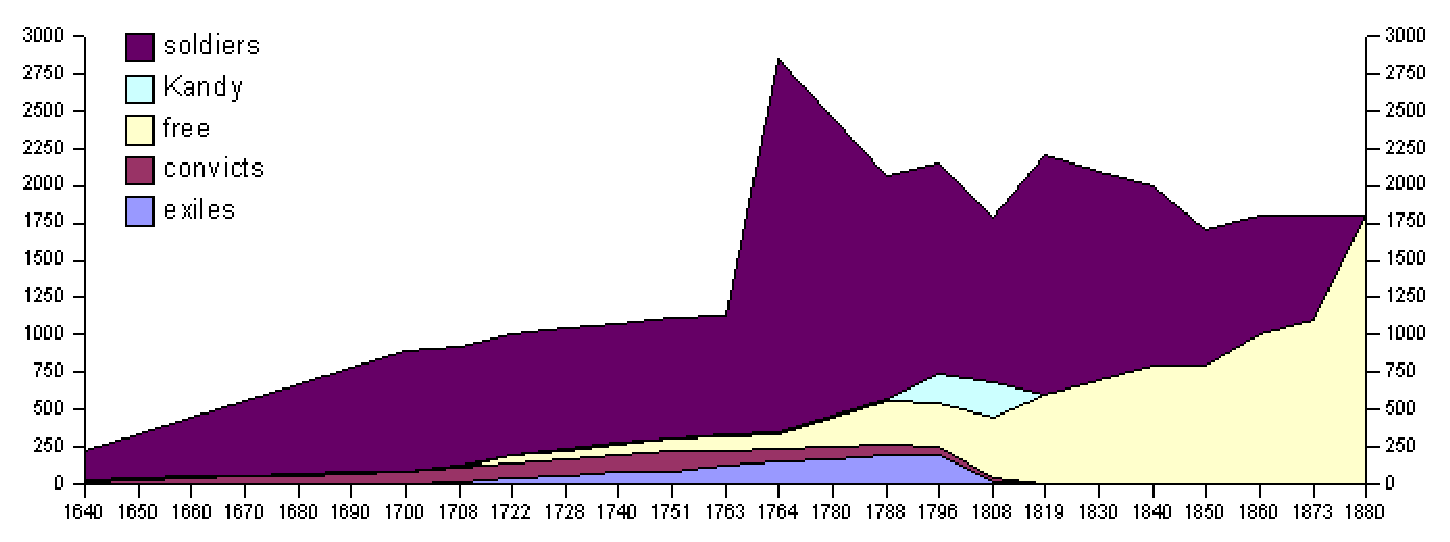
\includegraphics[width=1.00\textwidth]{pics/malaypopovertime}
	\caption[Development of the Malay population in Lanka over time]{The development of the Malay population in Lanka over time. Data are scarce and unreliable. Data for soldiers are good from 1764 onwards, the other groups are mostly based on two or three years where information is available and linear grow or decrease to/from this years. Furthermore, there is virtually no information about women, so the diagram is to be taken with a huge grain of salt. Sure points are the beginning and end of exile population, short intermittance of Kandy Malays and the grow of the free Malay population after 1796 to the detriment of the soldier population.}
	\label{fig:malaypopovertime}
\end{figure}


The subsequent recruitments were done in the Malay peninsula and were a lot less massive. The recruits came in a much more trickling way of about 40 a year with  peaks in 1819 and 1834 attaining 100. It can be assumed that they had to adapt to the linguistic usages of a Regiment with established ranks and norms.

%If, in order to have a good base for a comparison, we only consider the recruits, and not the wives and children, 647 recruits came from the SEAA and 698 from the Malay peninsula.\footnote{ This disregards the Malays brought from Cochin/India.}. We see that the amounts are about even. The peninsular recruits would have spoken some form of Malay at arrival \kuckn whereas the recruits from the SEAA would have spoken some form of SJKHDSFD\kuckn. The recruits from the peninsula are said to be of ``low quality''  \citep{abc} . It is thus not very likely that they had high prestige and others would imitate their speech. As for absolute numbers, they matched the newcomers from the SEAA, but were few against the already established Malays, who have their origins not on the peninsula. An important influence of the peninsular variety of Malay is thus not to be expected.
%
%There are some records of recruits from abroad having brought their wives and children. This was encouraged by the British \citet[12,52]{Hussainmiya1987}. It is thus to be estimated that the number of immigrants is much higher than the mere number of recruited soldiers. \draftnote{sch�zen}

After the Regiment had  plunged to 1000 men in 1850, the rules of the regiment were changed and allowed henceforth retirement after 15 years of service. Few Malays made use of this and went back to Singapore or Penang. A serious impact on the Malay society in Lanka is not to be suspected by these few returnees.

In Colombo and Kandy, the Malays were numerous enough to populate entire quarters of the town, Katukelle in Kandy and Slave Island in Colombo  where they had Moors as their neighbors \citep[111f]{Hussainmiya1990}.


\begin{quote}
    ``Further investigation is necessary to confirm whether the Dutch also followed a similar policy. In any case, the number of women arriving from the East Indies was limited, as a good proportion of 'Malay' soldiers had to find their wives among the local women from the Sinhalese, Tamil or Moor communities. It appears that the Malay Muslims preferred to marry the local Moor women because of their common religious background. A number of such cases of intermarriage between the Malays and the Moors is reported in the Tombos'' \citep[52]{Hussainmiya1987}
\end{quote}



\subsubsection{Demographic history after the disbandment of the Regiment}\label{sec:slmbg:DemographichistoryafterthedisbandmentoftheRegiment}
The disbandment of the regiment has not had a great impact on the composition of the Malay population in Sri Lanka. Only 80 Malays went back to Singapore \citep[104]{Hussainmiya1990}. But there were no more new recruits from the East bringing fresh blood and new cultural developments to Lanka. This lacking cohesion was detrimental to the Malay society. And while the number could be maintained, the degree of internal organization and cohesion was a lot less than during the CRR's days. The families had lost their great point of common interest, and the new jobs in the police or on the plantations involved work on a smaller scale in which one would meet a lot less Malays every day than before.
Even if many Malays served in the police, it was not an exclusive Malay domain like the Regiment, and Sinhala or Tamil officers would have forced the use of English, Sinhalese or Tamil in the office. Furthermore, the critical mass for maintaining a language might not have been attained by the smaller police stations.

%\begin{quote}
% %   [After disbandment, ~500 Malays in police]\citep[103]{Hussainmiya1990}
%\end{quote}

\subsubsection{Conclusion}\label{sec:slmbg:british:demographic:conclusion:Conclusion}
During the time of the Regiment, the Malay saw an important
portion of their fellows leave, the aristocrats sent back in 1808.
Governor Maitland did not recruit more Malays, which had the
number of enlisted Malays sink to 800. Governor Brownrigg wanted a
strong Malay Regiment and perpetrated a massive recruitment, first
from Java and after the British had lost Java, from Penang and
Singapore. Until 1819, 1016 new recruits joined the ranks of the
Sri Lanka Malays, about evenly from Java and the peninsula. The
Javanese were regarded higher though \citep[93f]{Hussainmiya1990}. These are likely to have
perturbed the established linguistic setting because of their
punctuated arrival and their higher prestige.

It was more and more difficult to find recruits in the East. The
number of soldiers decreased. After 25 years without bellicose
activity, the CRR was disbanded. While this did not entail a
back-migration to the SEAA, it stopped the arrival of ``fresh
blood'' to Lanka and deprived the Malays of an important domain
for using the Malay language.

\subsection{Sociological History under the British}\label{sec:slmbg:SociologicalHistoryundertheBritish}

\subsubsection{general}\label{sec:slmbg:general}
The Sri Lanka Malays can be said to have developed a distinct
identity in the beginning of the 19th century both different from
Lankans and Malays in the SEAA \citep[11]{Hussainmiya1987}. Their
small community was organized around the military service with the
exiles being cultural and spiritual leaders that sometimes also
served in the regiment. The Malays are known for their zeal that
exceeds the Sinhalese's and the Moors'. The exiles formed an
important part of the Malay society and they ``lent a certain
amount of cohesion, reflected glory and guidance to its
members''\citep[79]{Hussainmiya1990}, but a good part of them was
sent back in 1808. The military officers then assumed the role of
community leaders. They were well respected in the Regiment, even
among British officers, as well as in the community. Until about
1850 the Regiment formed a central part of the Malay society with
everything revolving around it. Security, solidarity and
understanding among the families characterized the life in the
cantonment. The houses were built close to the military
administration center, as was the mosque where worships were held
in the Malay language. Children could attend the school of the
Regiment and become half-pay boys later before entering the ranks
of the CRR whereas old people were taken care of by the Invalids'
Company. Intermarriage among the Regiment was frequent and the
social status of a community member could be evaluated by the
number of officers attending his wedding. \draftnote{or rank or
name}

The attractiveness of the Regiment began to decline in the 1820s.
After 1850, with a low pay and service in Hongkong making the
Regiment unpopular, the number of free Malays (\em Orang
Priman\em) went up. The \em Orang Priman \em chose jobs from the
domains of the police, the firemen, other security related jobs,
plantations, departments and offices \citep[90]{Hussainmiya1990}.

The cultural leadership of the Regiment was challenged towards the
end of the CRR (1873). In an argument about the position of the
Imam in the Malay mosques, the soldiers could not impose their
candidate, and a certain kind of schism occurred with military
Malays and civilians attending different services
\citet[125]{Hussainmiya1990}.

During the time of the Regiment, the Malays lived in some kind of
more or less autarkic community in the garrisons and their
isolation aided the preservation of their identity. The Regiment
provided everything they needed, from quarters for married
soldiers to the military school to the mosque.


Trips to their homelands were also not unknown of.



%\begin{quote}
%   ``A few members of the exiled Royal families seemed to have stayed behind, especially those who married local women. \el the often-claimed princely ancestry of many later day Sri Lankan Malays can rarely be \el substantiated with any credibility''\citep[61]{Hussainmiya1987}
%\end{quote}

\subsubsection{Regiment}\label{sec:slmbg:Regiment}
The Malays were highly regarded in the regiment, also by the British officers. A career from a half-pay-boy to a captain was possible, contrary to European officers, who were taken from the military academy and never from the low ranks \citep[122]{Hussainmiya1990}.

The Regiment was bound by strong kinship ties. Many Malay families depended on the regiment as their only source of income \citep[78]{Hussainmiya1990} and soldiers joined because of family tradition. The Malay network was tightly knit and the Malays had a certain feeling of superiority regarding the Sepoys and Kaffirs\draftnote{and also the Sinhalese and Tamils??}.



The Regiment cared not only for the active soldiers. Retired soldiers were either given land in the south or cash money. Taking land in the south does not seem to have been very popular with the Malays because it would have removed them from there community. Unless the land was close to the cantonment (for instance \em Kampung Pensen \em in Kandy), the Malay preferred the money.

While the Regiment provided cultural and religious support for the Malays, the actual living conditions of the soldiers seem  to have been pretty poor. We  only have good  knowledge about the sociological circumstances of the Malays living in Colombo and Kandy. But in the South, things seem to have been worse and soldiers are said to have lived in ``wretched huts'' \cite[115f]{Hussainmiya1990}.

\begin{quote}
    [regulations and wages \citep[60]{Hussainmiya1987}]
\end{quote}

\subsubsection{School}\label{sec:slmbg:School}
In 1812, the first military school for Malay boys was founded. Their number rose to 5 until 1860 \citep[99]{Hussainmiya1990}. The goal of the school was to provide good education to the ranks of the Malays. \kuckn Officers could order their soldiers to attend school. Even if parents were not in the military, they could sent their children to this regimental school, what many did. The education provided was excellent and included Malay language, Tamil and English, but no Christian religious education  \citep[96]{Hussainmiya1990}. In the 19th century, the literacy rate among Malays was the highest among all ethnic group in Ceylon (\citet[48]{Marga1988}, cited after\citet[17]{Bichsel}). There are some numbers of the students attending the regimental schools:
    ``In 1835 there were 149 Malay boys studying at military school belonging to the CRR \el in 1873, when the CRR was disbanded it was said that there were 269 half pay boys serving the regiment''\citep[97]{Hussainmiya1990}. In 1872, shortly before the Regiment was disbanded, the enrolment was 391 \citep[17]{Bichsel}. If we consider the falling number of soldiers in the late 19th century, it is impressive that there were still that many students in the Regimental schools. This must be due to civilian Malays sending their children to the Regimental schools as well.

\subsubsection{Work}\label{sec:slmbg:Work}
Civilian Malays would engage in the following occupations:
      civilian government departments,
      private business establishments,
      private European plantations,
      civil police department,
      district government agent's establishment,
      coffee and sugar plantations as overseers, conductors, security guards, tea-makers,
      servants,
      gardeners,
      rattan weavers,
      clerks,
      peons,
      book-keepers.

Police service proved particularly popular, maybe because of the
similarity to military work. 90\% of the police sergeants in
Colombo were Malay in 1833. After the coffeeblight in 1872,
cultivation of tea began in Ceylon. The Malays found work in the
new estates and in the railway construction companies that
connected the highland to Colombo. But contrary to the work in the
Colombo police force, the Malays were more of a minority in the
countryside. For instance, they were outnumbered by the Indian
Coolies in the tea estates \citep[90f]{Hussainmiya1990}.

\subsubsection{Faith}\label{sec:slmbg:Faith}
The British fostered the religion of the Malays and provided a
good infrastructure. There were special Malay mosques next to the
cantonments. This aided the cohesion of the community. Services in
the Moor mosques were  unpopular because the service there was
held in Tamil and Arabic, which did not suit the Malays. This also
sheds doubt on the pretended strong link with the Tamil Moor
community. The mosques did not only serve as a place for religious
meetings. Public meetings could also be held in mosques, also in
Malay language. Malay mosques existed in Galle, Trincomalee,
Kalpitiya, Badulla, Kirinda, Kurunegala and Kandy
\citep[124]{Hussainmiya1990} and Wekande,
Colombo\citep[126f]{Hussainmiya1990}\draftnote{and maybe more}

\begin{figure}
    \centering
        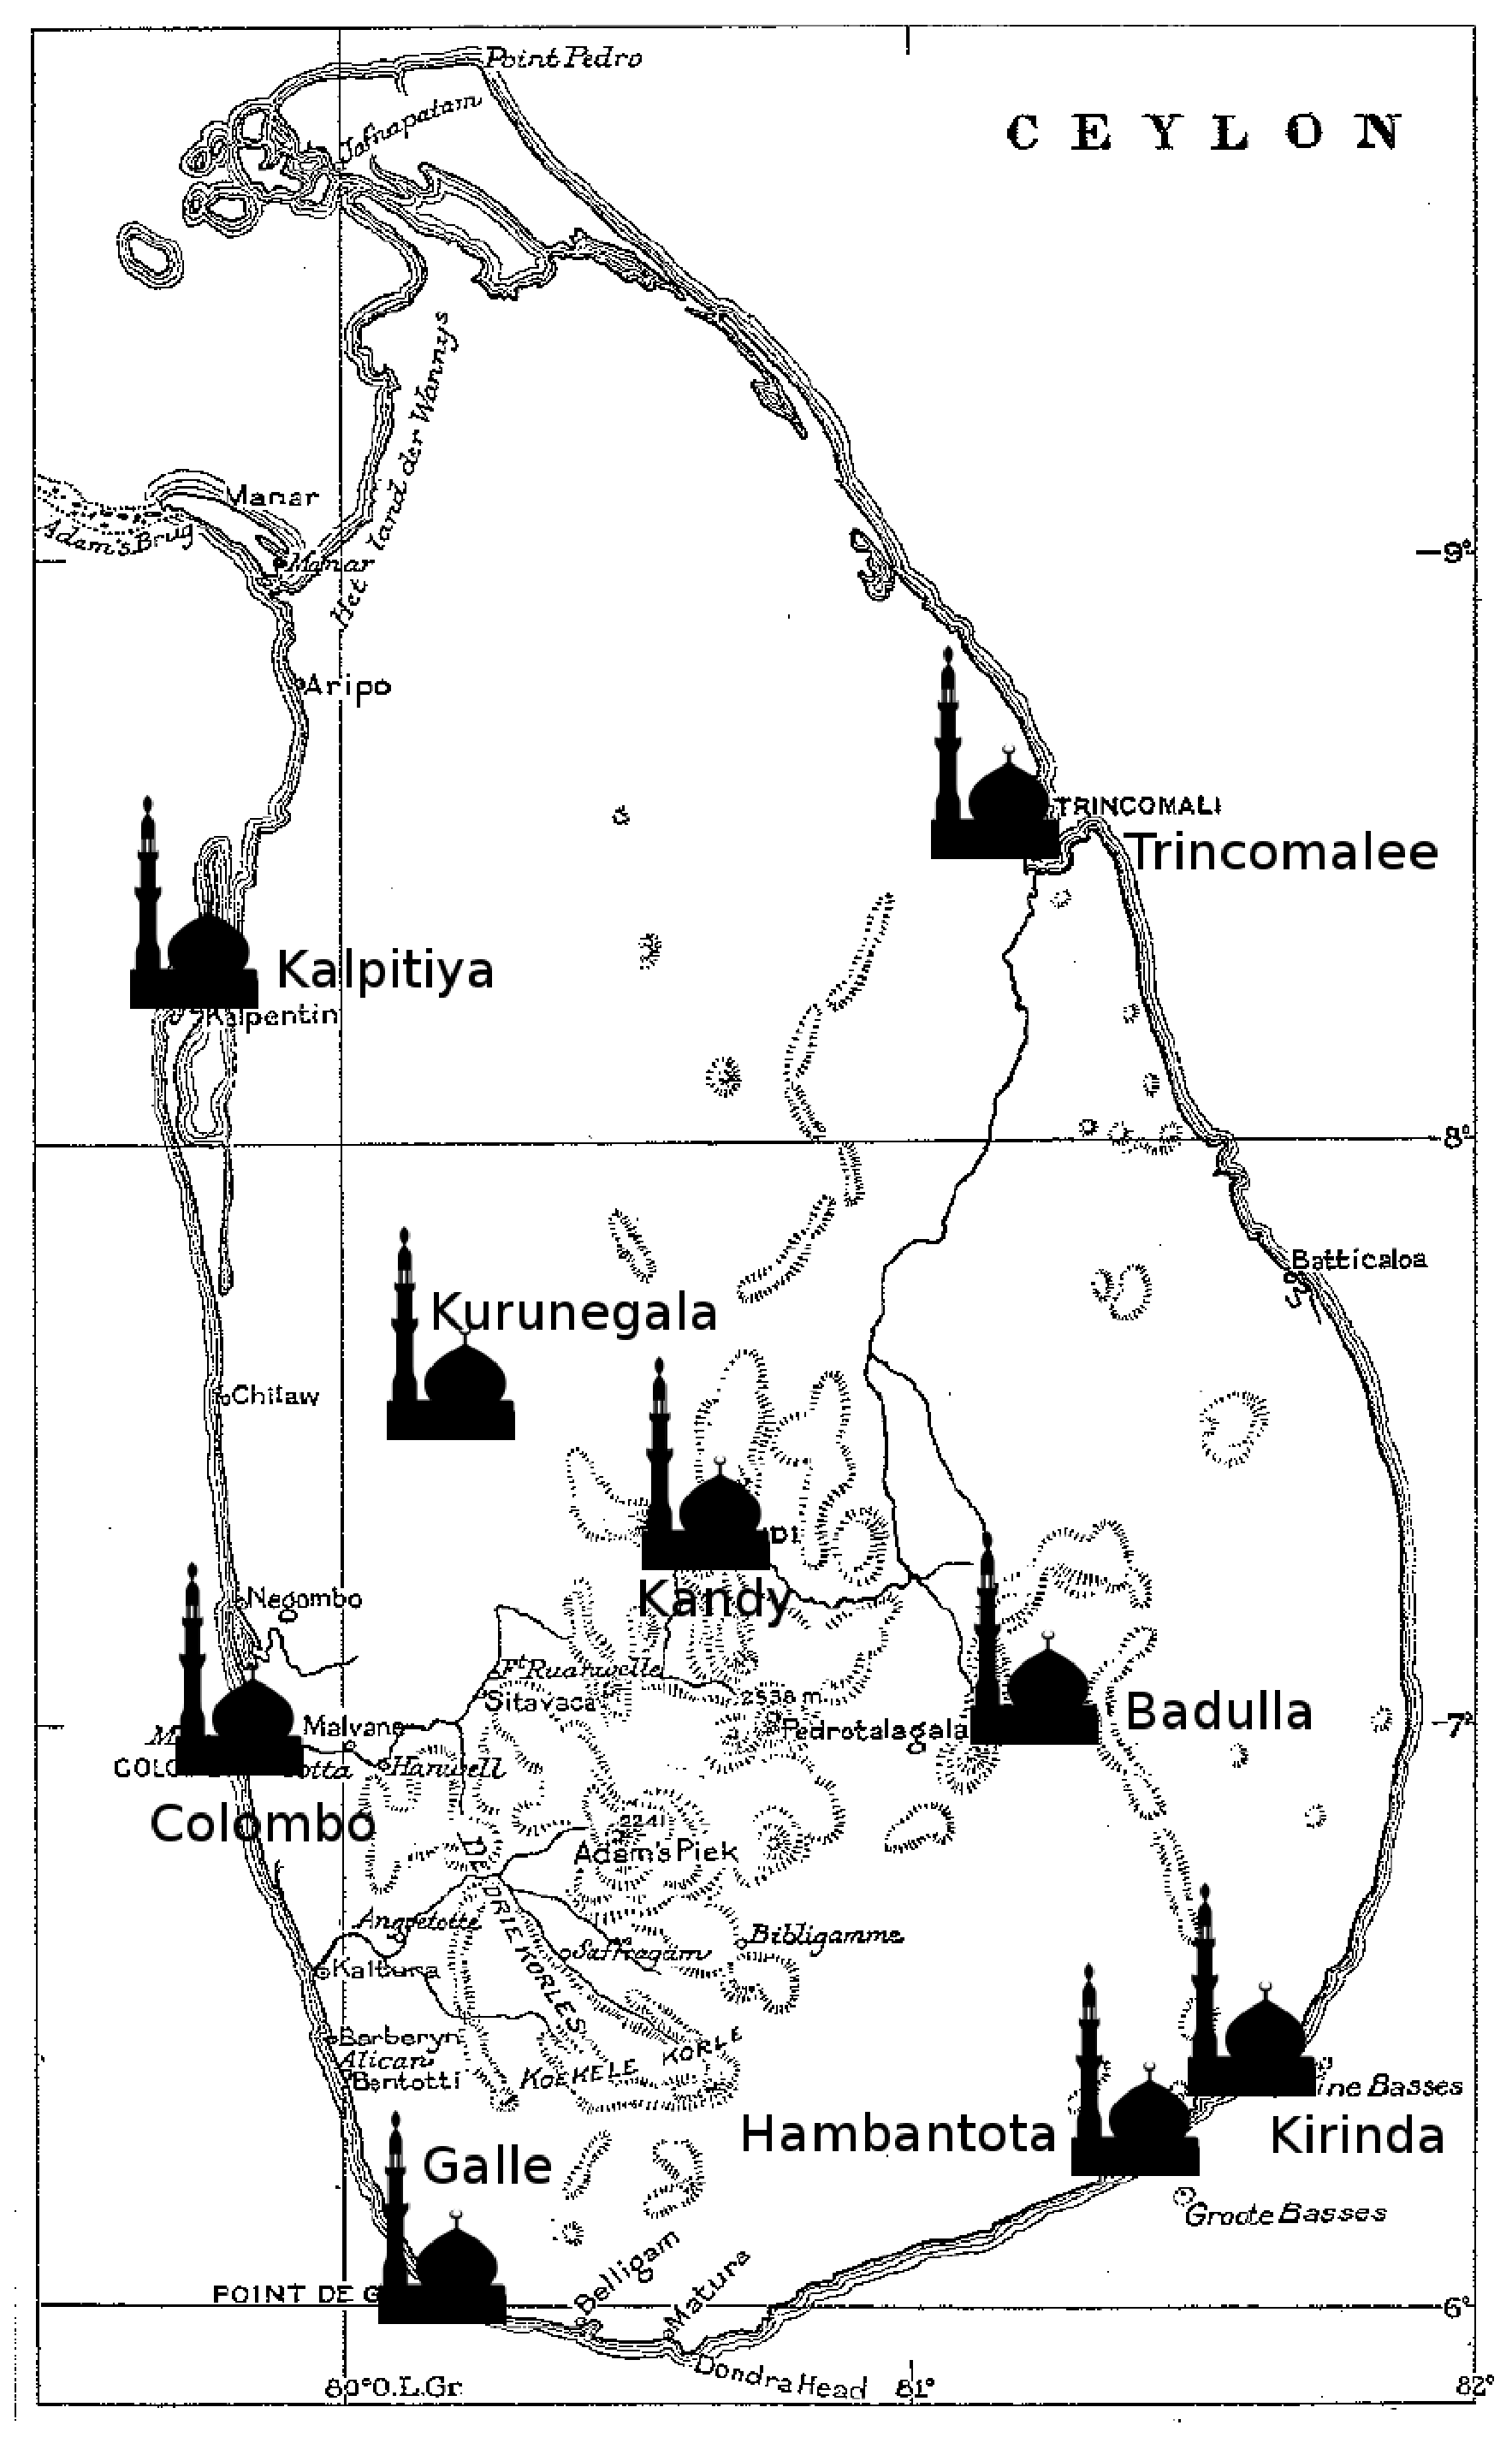
\includegraphics[height=.3\textheight]{pics/malaymosque}
    \label{fig:malaymosques}
\end{figure}

\subsubsection{Intermarriage}\label{sec:slmbg:Intermarriage}
\citet[119]{Hussainmiya1990} about intermarriage in the Regiment. No moors

\subsubsection{Art}\label{sec:slmbg:Art}
Within the protected environment of the Regiment, Malay officers
devoted themselves to fine arts and literature and assumed thus
the role that the exiles had had for the community before they had
been sent back to the SEAA.  The officers had a library equipped
with Malay books \citep[145f]{Hussainmiya1990} and a club where
the literature enthusiasts could meet. The works available are A
BC  and D and are discussed in \citet{Hussainmiya1987}. As a side
note, the CRR is likely to have created the first Malay library in
the Malay world \citep[146]{Hussainmiya1990}.

After retirement, the officers would still frequent their old
colleagues in the library room and cultivate literature. After the
disbandment of the regiment, they continued to meet, \kuckn but no
younger Malays joined them and when they died the use of Malay as
a literary language in Ceylon died with them. There are some
subsequent attempts to produce Malay literature, but they could
not meet the standards set by the officers.
\citet[130]{Hussainmiya1990}  sees them as  ``the last bastion of
the traditional Malay society symbolized in the institutions of
the CRR''.

%\begin{quote}
%   ``By helping the soldiers to run their own recreation room, which also served as a repository of books, the Regiment can be given the credit for establishing the first Malay library of its kind in the Malay world''\citep[146]{Hussainmiya1990}
%\end{quote}
%club

\subsubsection{Contacts with the SEAA}\label{sec:slmbg:ContactswiththeSEAA}
The Malays had regular contact with the SEAA during the 19th century. While they had a distinct identity, they had not forgotten their roots, and the new recruits arriving mainly in the first half of the century assured that the ties would not weaken. The recruiting missions were often accompanied by Malay officers and    ``some members of such recruiting missions stayed long enough in the peninsula, at times more than two to three years at a stretch, to bring back not only new developments in Malay culture, but also Malay literate texts and manuscripts to be distributed in their community''\citep[13]{Hussainmiya1987}. Hussainmiya also affirms that the Malays enjoyed visiting Penang, Malacca and Singapore. It is not entirely clear whether he sees this as some kind of tourism, or whether he refers to the recruiting officers\kuckn.

\begin{quote}
    ``even after the disbandment of the Ceylon Rifle Regiment in 1873, which had effectively put a stop to direct links with the peninsula, determined efforts by some members of traditional Malay elites in Sri Lanka, such as Baba Ounus Saldin (b. 1838 - d. 1906) prolonged some form of cultural links with Malayan archipelago until the very late part of the 19th century''\citet[13]{Hussainmiya1987}
\end{quote}

\begin{quotation}
    ``[The disbandment of the CRR] can hardly be considered the type of revolutionary change required for rapid contact-induced change''\citet[19]{SmithRH}
\end{quotation}

\section{Postregimental History}\label{sec:slmbg:PostregimentalHistory}
\subsection{Ereignisgeschichte}\label{sec:slmbg:postreg:Ereignisgeschichte}
The early twentieth century saw the rise of the movement for independence as well as the rise of communalism of the different ethnic groups in Sri Lanka, most notably the Tamils' \citep{abc} . The Malay community, too, formed a political association for the first time and demanded representation \citep{abc} . This cannot betray the fact that the importance and internal cohesion of the Malay community decreased, which can be seen in the switch of more and more mosque services from Malay to Tamil  \citep{abc} .
From 1924 to 1965, the Malays had an appointed MP in parliament, who was not elected by universal suffrage but rather appointed by the government to represent the minority of the Malays. The Malays' representative was TB Jayah, who enjoys a lot of prestige still today and is commemorated by the TB Jayah day on the 3rd of December\kuckn. TB Jayah was also part of the delegation negotiating the terms of independence with the British. in the 1950s, the 2500th anniversary of the Buddha \kuckn let to increased communal consciousness among the Sinhala, who asked for a greater representation in society which would reflect their status as the majority ethnic group. Up to now, the higher strata of society had been dominated by Tamils or Burghers. The Sinhala used their majority in parliament to vote a number of laws favouring their group, on university access, number plates on cars and finally the infamous `Sinhala only' law, making Sinhala the sole official language of the country, which was resented by the other communities and fueled the ethnic tensions \citep{abc} . As for the Malays, the mandatory use of Sinhala in the education system meant that they had to devote more time to that language than before, when they had mainly functioned in SLM at home and English in education. This caused a sort of chain reaction, where Sinhala pushed English out of the educational systems, and the Malays, who wanted to preserve their superior command of English as compared to the other groups chose to educate their children in English, which in turn pushed SLM out of that domain.

The ethnic tensions between Tamils and Sinhalese lead to the outbreak of open civil war in the 1980s, which in turn lead again to a rise of ethnic consciousness in the other groups and culminated in the creation of the SLAMAC (Sri Lankan Malay Confederation) on 18 August 1985, four years later than the establishment of the Sri Lanka Muslim Congress (SLMC), which is mainly supported by Moors.

In the early 1990s, the Malays would yet again be represented in parliament, when MH Aamith was appointed MP by the then Prime Minister \kuckn Premadasa.


 The Moors were able to turn the SLMC into a political party with some influence, with as one of the consequences that in the recent census(es)\kuckn, Malays and Moors are now subsumed under the ethnic [sic] group ``Muslims''. This makes future representation of the Malays in parliament unlikely, since their ethnic group of ``Muslims'' is already represented in parliament by the SLMC, even if all of the members are Moors, whose interests very often diverge from the Malays'. This arrogation \kuckn of voice of all Muslims by the Moors has led to irritation within the Malay community, who do not feel that the Moors can speak on their behalf, albeit that they are Muslims.






\begin{quote}
    ``In Sri Lanka, after neatly a century of British rule, nationalist fervor had been on the rise''\citet[15]{Hussainmiya1987}
\end{quote}

\begin{quote}
    ``One was the nationalist wing, who endeavoured to accord greater prominence to the cultural patterns and religious traditions of the country; while the constitutionalists stood for a limited programme of political freedom, though not bargaining for a total disturbance of the main features of the British colonial hold od the island.''\citet[15]{Hussainmiya1987}
\end{quote}

\begin{quote}
    ``For the first time the local 'Malay elites', though a miniscule [sic] minority, began to demand their own political rights in Sri Lanka, the country of their adoption, when they felt the opportunity to claim a seat in the legislative council''\citet[15f]{Hussainmiya1987}
\end{quote}

\begin{quote}
    ``The greatest concern of the minority of Malays was that their ethnicity and identity was getting over-shadowed by the numerically superior Muslim-Moor group.''\citet[16]{Hussainmiya1987}
\end{quote}

\begin{quote}
    ``The period between 1920 -- 1930 constitutes a watershed in the evolution of ethnic-consciousness among the Malays of Sri Lanka. They decided to form a political association for the first time \el The motive was to urge the British authorities to concede a Malay seat in the legislative council.''\citet[16]{Hussainmiya1987}
\end{quote}

\begin{quote}
    [in 1921there are still Malay mosques in 1921]
\end{quote}

\begin{quote}
    ``The political-identity crisis for the Malays also brought in its wake a strong desire to revive the community's cultural past which had been in the process of slowly being discarded.''\citet[16f]{Hussainmiya1987}
\end{quote}

\begin{quote}
    ``during the golden Jubilee year of the Colombo Malay Cricket Club in 1922, the Malays decided to widen the scope of a communal association by founding an all Ceylon Malay association with the view to cater to the cultural, economic and religious needs of the community''\citet[16f]{Hussainmiya1987}
\end{quote}

\begin{quote}
    ``The Malays' desire to assert their special heritage has been pursued relentlessly since then by various means, by organizing public lectures on their history, by activating special committees to conduct archival research on their past to search and revive their original Malay Jawi, and Javanese script, to publish books in Malay and to conduct special classes in Malay language etc.''\citet[18]{Hussainmiya1987}
\end{quote}

\begin{quote}
    ``In any case the right to send one of their own men to the legislative council was conceded to the Malays, and from 1924 to 1952 at least one Malay was chosen to represent the community's interests, in 1952, they temporarily lost the Malay representative in the Parliament, but through the six special seats allotted for special interests in the Ceylon Parliament in accordance with the provision of the Soulbarry constitution of 1948, a Malay member was nominated to the parliament but only until 1965. Since that year, no Malay member was nominated even for a special seat. The Malays lost this privilege of a nominated member of the parliament with the introduction of a new constitution in 1972.\el The significance of Malay political representation in strengtheni
\subsubsection{Tsunami}\label{sec:slmbg:Tsunami}
ng their communal identity in Sri Lanka cannot be underestimated.''\citet[20]{Hussainmiya1987}
\end{quote}

\begin{quote}
    ``Founded in 1922, the All Ceylon Malay Association (ACMA) had been a principal rallyi[n]g force of the community. [Its] headquarters is situated at Padang, in the heart of the Malay enclave of the Slave island area in Colombo, and its branches spread to other partes of Sri Lanka which have significant Malay population.''\citet[21]{Hussainmiya1987}
\end{quote}



\begin{quote}
    ``special committees were set up [by the ACMA] to collect oral and written literature; also Malay dancing and music were revived.''\citet[21]{Hussainmiya1987}
\end{quote}

\begin{quote}
    ``The loss of importance of the ACMA as the main Malay organisation during the last two decades, also symbolised perhaps the crisis in the ethnicity identity of the Malays.''\citet[21]{Hussainmiya1987}
\end{quote}

\begin{quote}
    ``aggravated demands for separation and self-rule on the part of the Tamils, a largest minority community Sri Lanka [sic], have spurred feverish activities on the part of all the communities to define their respective rights. The birth of a new umbrella Malay organization in 18 August 1985, SLAMAC, or Sri Lankan Malay Confederation (its Malay name being KORAMEL, Konfederasi Rakyat Melayu Langkapuri) can be seen as direct response to new political developments in Sri Lanka''\citet[22]{Hussainmiya1987}
\end{quote}

\begin{quote}
    [2nd  Malay world symposium in SL 1985]
\end{quote}

\subsection{Demographic postcolonial History}\label{sec:slmbg:DemographicpostcolonialHistory}
While Hussainmiya provides ample detail about the sociohistoric conditions in which the Malays evolved in the 19th century, information of comparable quality is not available for the 20th century because the Ceylon Rifle Regiment, Hussainmiya's object of study, had been disbanded by then. In what follows, I will sketch the sociohistorical and demographic history of the Upcountry Malays based on extended discussions with several older members of the Malay communities from Kandy, Gampola, Nawalapitiya, and Badulla.

The generation of Malays born around 1880 (thus the grandparents of the oldest speakers) chiefly worked in the army, law enforcement, the railway or as overseers on the estates. They went to mixed schools, where Malays, Sinhalese, Moors, Burghers and Tamils\footnote{Estate Tamils (Indian Tamils) or Ceylon Tamils).} were educated together. In one school, the first grades, classes were taught in Tamil with one subject being taught in English, while in the advanced grades, English was the medium of instruction\kuckn. Many schools were run by Irish nuns, where education was in English. A curious fact is that in one school, Islamic education was taught by Tamils from Jaffna, who were Hindus. Apparently, this did not pose a problem to either of the two communities. Schools could be as far away as 7 miles, requiring 2 hours of walk to reach them in the morning, and the same amount of time to get back home in the afternoon.

The main upcountry towns of Kandy, Nawalpitiya, Nuwara Eliya, Hatton and Badulla were by no means isolated and there were frequent contacts among inhabitants of different towns, which can be seen by the very common marriages involving partners from different towns. Marrying into a family of another town was a common practice (and still is today). This might have  helped preserve Upcountry Malay as a coherent variety with little internal diversification. As an interesting side effect, the idiolectal diversity we find in the Upcountry seems to be tied not to region but to family lines. For instance, one speaker from Kandy uses \phonet{a\E?d u:Du?} for the present tense from \trs{araduuduk}{is.sitting} even in careful speech, which is normally pronounced \phonet{ar\E du:duk}. This makes more sense if one knows that she was born in Badulla, but that her father was born in Hambantota in the South, where such contractions seem to be more common. The rest of her idiolect does not differ much from other idiolects from Kandy, but this one feature betrays the origin of her family in the South two generations earlier.

Contact with Colombo was also very frequent (at least after independence), and most Malays from Kandy have relatives in Colombo. Other than that, one speaker from Kandy had her mother from Negombo, to the North of Colombo, another one's mother is from Puttalam. The wide-spread kinship ties of the Malays prove that in the last three generations, the Malay network covered all of the Upcountry and Colombo/Negombo on the coast. It is less common to have relatives in the South (Hambantota, Kirinda); this community seems to form a separate network. There are some Malays in Galle, who still speak Malay, but who seem to be quite isolated from the rest. Figure \ref{fig:Kandynetwork} gives an impressionistic illustration of the perceived strength of ties. Further more sophisticated demographic research must show whether the postulated strength of ties holds up to statistical analyses.

Before independence, the Upcountry Malays had close ties with the Burghers on the estates and their style of life was comparable and less traditionalist than the style of life of the Moors. This is still the case today with the Malays being much more lenient with regard to the literal following of Islam teachings than the Moors, who tend to be more observant. Examples of this are the wearing of the veil, which is more common among Moor women than among Malay women, and the size of the veil, which tends to be less for Malays, if present at all. Regular attendance of religious services seems to be more important among the Moors than among the Malays. An additional factor which might influence this is that the services in the mosque are conducted in Tamil, which is understood by all Moors, but not by the younger generation of Malays. Not understanding the content of the sermon\kuckn obviously impedes the appreciation of the religious experience.

In the course of the twentieth century, the main fields of occupation of the Malays did not change, and various jobs in the maintenance of public order like the police, jail guards, firemen or soldiers remained popular. Given that after independence the Sinhalese acceeded to the ruling positions in these areas, the Malays loyalty now resides with them, and support for the actions of the Sri Lankan government and the Sri Lankan Army (both dominated by Sinhalese) in the civil war is widespread.\footnote{I do want to emphasize the complexity of the Sri Lankan society and stress that a simplistic equation government=Sinhala is not warranted. The government is not entirely constituted of Sinhalese, and its actions do not have the support of all Sinhalese.}

In recent years, however,  white-collar activities in the commercial sector seem to be increasing at the expense of the traditional occupations.

It is possible to marry members of other communities, but those are then required to convert to Islam if they were following another religion before. As a rough estimate, about 10\% of marriages involve a member of the Moor community and 5\% involve a member of the Sinhala Buddhist community. Marriages to either Hindus or Christian is very uncommon. 





\begin{figure}
 \centering
 
\includegraphics[height=0.3\textheight]{pics/Kandy-network}
 % Kandy-network.jpg: 478x600 pixel, 362dpi, 3.35x4.21 cm, bb=0 0 95 119
 \caption[Strength of contacts between Kandy and other towns]{Impressionistic strength of contacts between Kandy and other towns, and between Badulla and the South}
 \label{fig:Kandynetwork}
\end{figure}






\subsection{Sociological History}\label{sec:slmbg:SociologicalHistory}

\begin{quote}
	``networks chiefly constituted of strong ties support minority languages resisting institutional pressures to languge shift; but when these networks weaken, language shift is likely to take place''\citep[124]{MilroyEtAl2003}
\end{quote}

\begin{quotation}
    ``[F]rom the 1930s , female participation in the educational system increased, producing more bilingualism among women; also from the 1930s, Tamil began to replace Malay in the mosques and other religious contexts; after independence in 1948, the importance of Sinhala for government related employment and the fact that English-medium education was no longer available in the public system made many Malay families opt to send their children to Sinhala medium schools''\citet[3]{SmithEtAl2004}
\end{quotation}


The Malays are quite well integrated into the Sri Lankan society and participate in all walks of life up to the topmost strata, including national sportsmen, ministers, film stars, singers, media presenters, the most famous journalists, high representatives of Sri Lankan Airlines
\section{Malay settlements}\label{sec:slmbg:Malaysettlements}
Being mercenaries, the Malays had always lived close to the centers of colonial power when they were not engaged in military campaigns. The native Lankan population was much more dispersed, and even today, Sri Lanka is not a very much urbanized country\footnote{   \url{http://www.nationmaster.com/graph-T/peo_per_liv_in_urb_are}.} Also the exiles were confined to the centers of colonial power because they had to be under control of the authorities. This urban base distinguishes the Malays from the Sinhalese and Tamil Hindus, and to a lesser degree from the Moors.

During Dutch times, Malay regiments were stationed in the four main coastal towns of Colombo, Galle, Trincomalee and Chillaw \citep{abc} .
Kandy was still independent during that time, but had a certain population of deserted Malays.
After the British had vanquished the Dutch and the Kandyans, the main Malay settlements were Colombo and Kandy. The first non-military settlement was founded in 1802, Hambantota, where retired Malays were given land to cultivate\kuckn. This colony  was followed shortly by Kirinda and Palatupana not far away.

Beside Colombo, Kandy and the South, there were further
detachments in the towns already inhabited by Malays during Dutch
times and in Badulla, that had been under Kandyan rulership until
18XX. \kuckn Following the 1848 rebellion, special detachments
were set up in Kurunegala and Matale In 1860, there were 5
companies in Colombo, 3 in Kandy, 2 in Galle, 2 in Trincomalee,
one in Badulla, and  the Sepoy company in Jaffna. In addition,
detachments of soldiers from Colombo or Kandy or Galle were sent
to Puttalam, Kurunegala, Hambantota and Chillaw. Figure
\ref{fig:malaypop1860} shows the towns where the Malays were
placed in 1860. In 1865 the Military Commission recommended the
closing of all CRR stations for reasons of economy, except those
of Colombo, Kandy, Galle, and Trincomalee.\draftnote{plag}

\begin{figure}
    \centering
        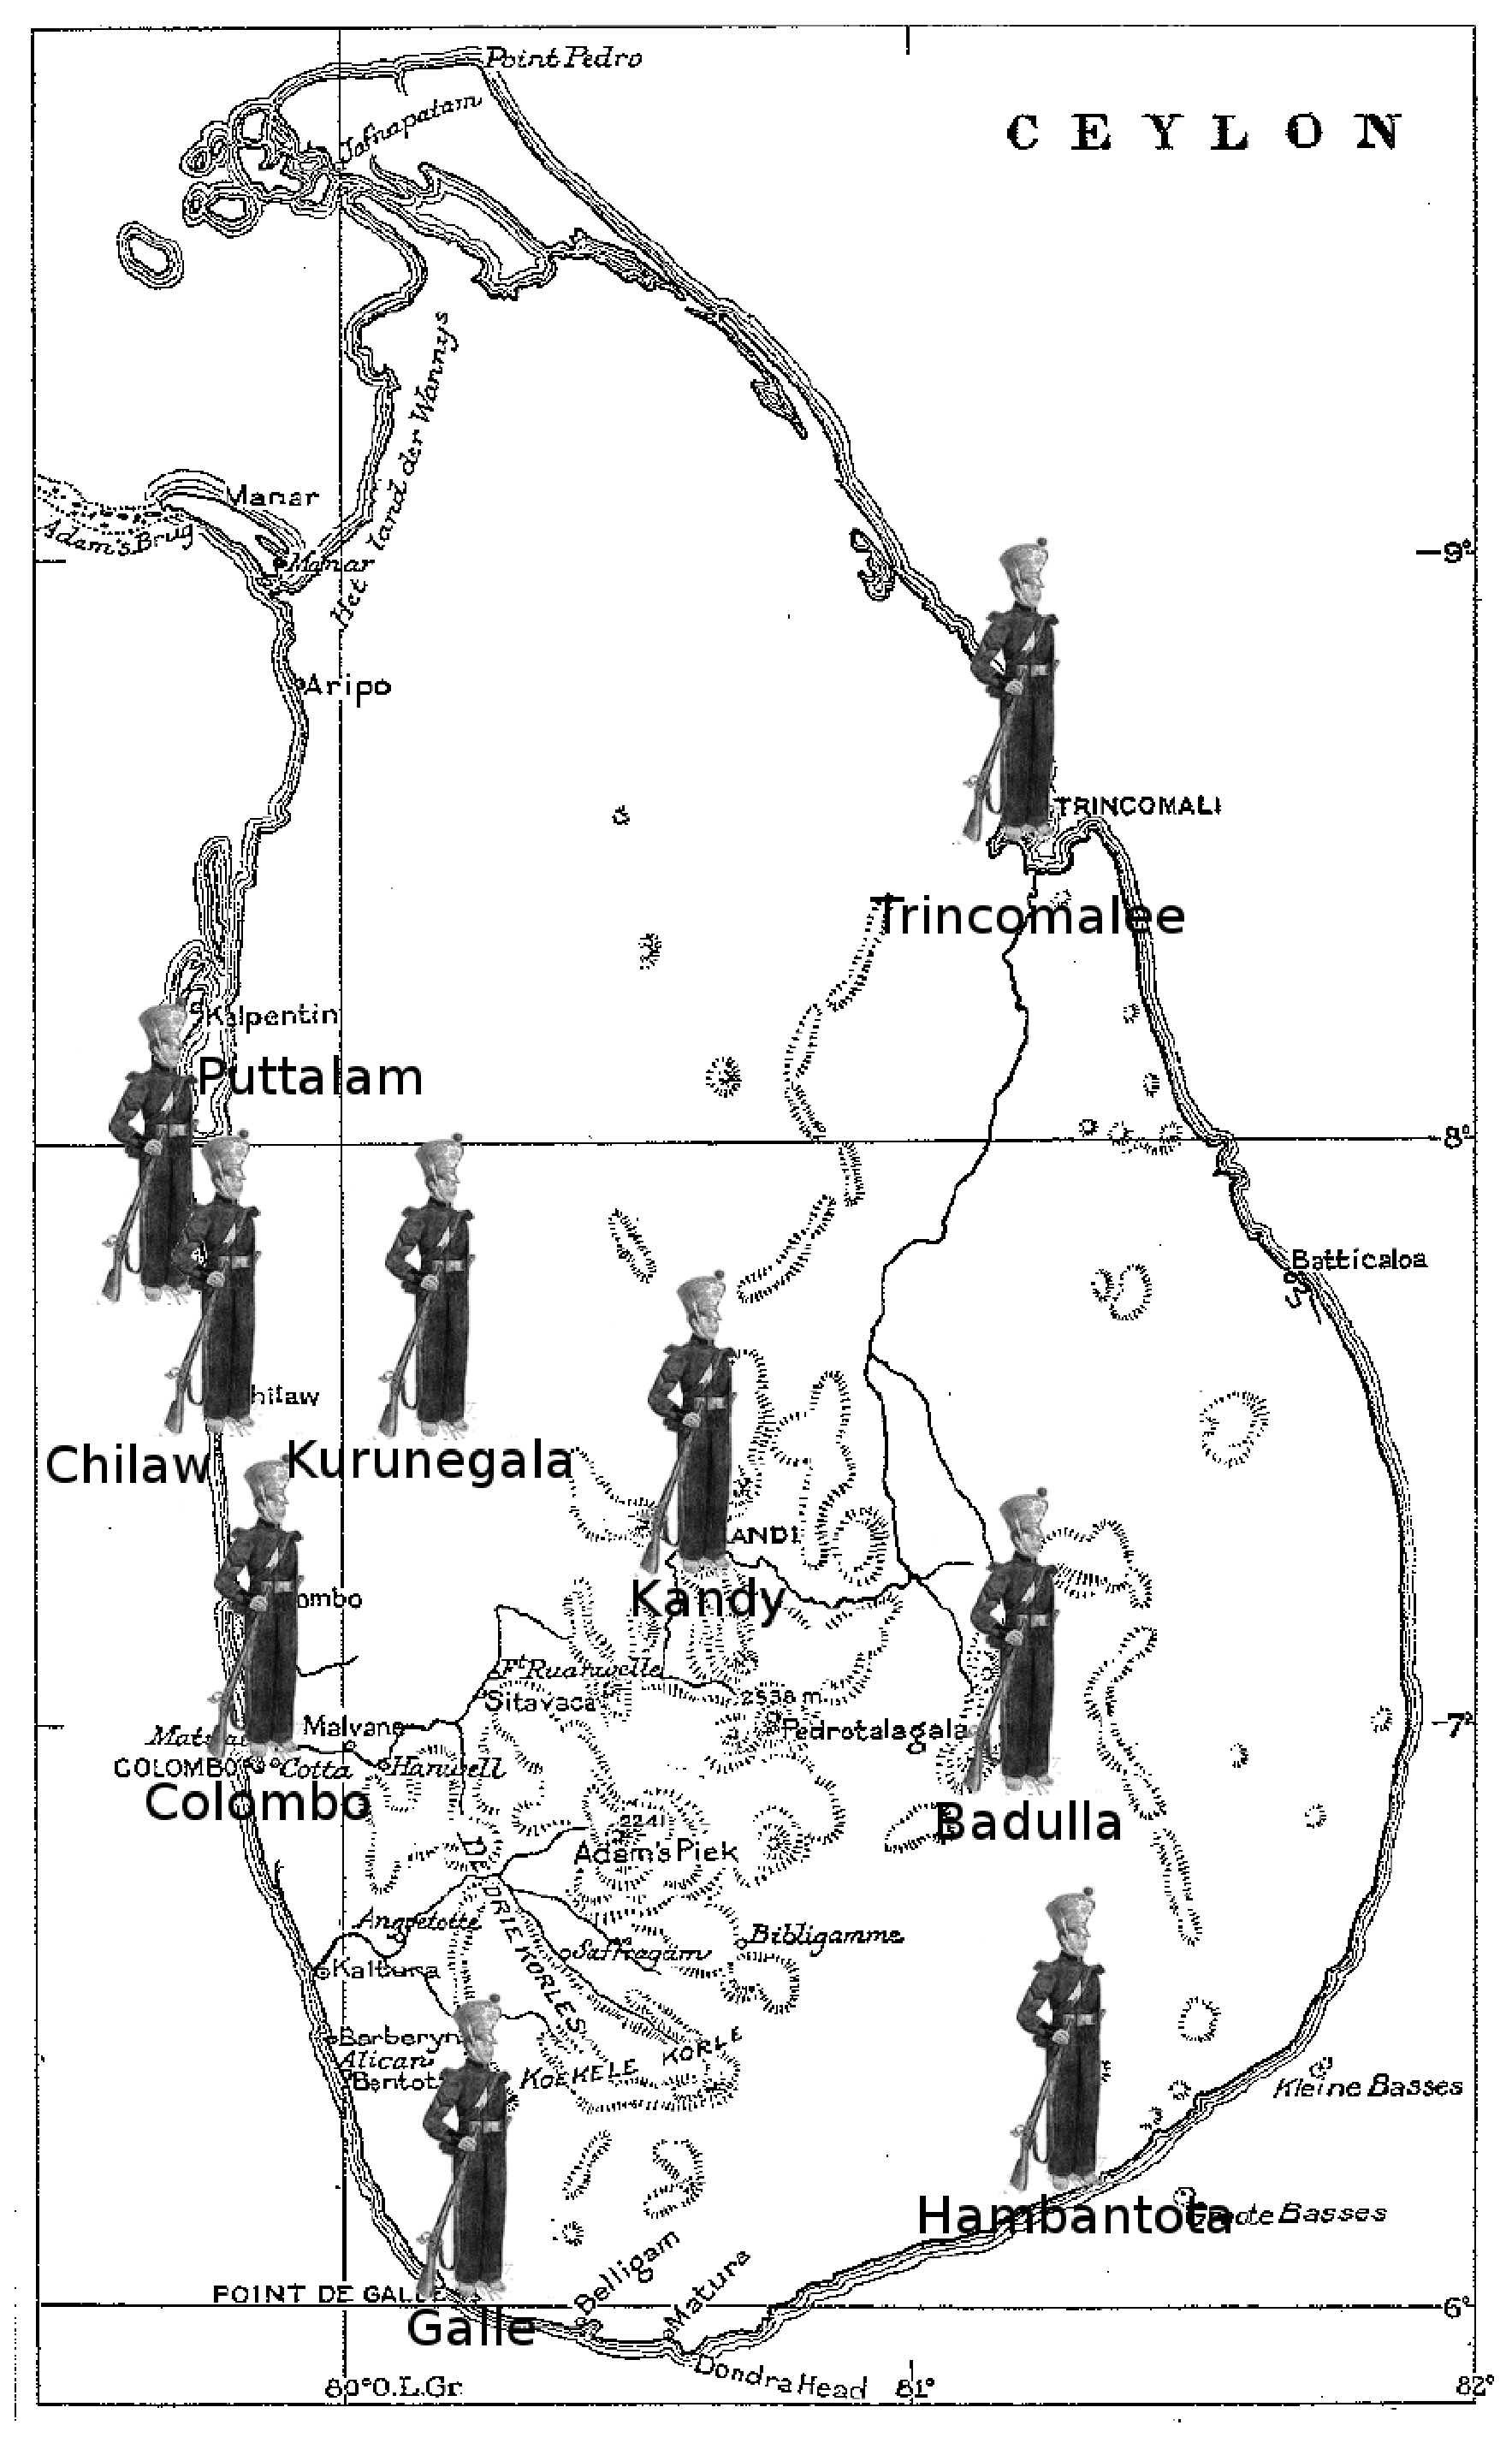
\includegraphics[height=0.3\textheight]{pics/malaycomp}
    \caption{Malay companies or detachments in 1860}
    \label{fig:malaypop1860}
\end{figure}

According to Bichsel-Stettner, the Malay population concentrates in the population centers given in table \ref{tab:MalayPopCtr}.
\begin{table}
    \centering
        \begin{tabular}{lrr}
          & Town & Population\\
        \hline
        1 & Colombo & 20.041\\
        2 & Gampaha & 8.077\\
        3 & Hambantota & 4.380\\
        4 & Kandy & 2.648\\
        5 & Badulla & 1.300\\
        6 & Kurunegala & 1.201\\
        7 & Nuwara Eliya & 1.113\\
        \end{tabular}
        \caption{Population centers with Malay population}
        \label{tab:MalayPopCtr}
\end{table}

\subsection{Colombo I}\label{sec:slmbg:ColomboI}

Inside Colombo, there were two main quarters for Malays, which were home to the different ethnic groups, i.e. common Malays in Wolfendhal and exiles in the adjoining quarter known as \em Kampung Pangeran \em or Princes' quarters. While being geographically separate, they still lived close enough to interact.

In the beginning of the 19th century, Slave island (aka \em Kampung Kertel \em) became an important Malay quarter in Colombo following the installation of an administrative block, officers' mess, married men's quarters, a bachelors' mess, military school, and a parade ground.

\begin{figure}
    \centering
        \includegraphics[width=0.60\textwidth]{pics/colombomod}
    \label{fig:colombomod}
\end{figure}

\begin{quotation}
    ``Place names in and around Colombo such as Malay Street, Java Lane, Jawatte (`Java Garden') Road and Jaela (`Java-Stream') signal the Malay presence on the Island.''\citet[12]{Jayasuriya2002}
\end{quotation}

After the dissolution of the Regiment, the Malays were each given a piece of land in the Cinnamon Jungle
Malays sell their houses to buy less expensive land in areas such as Wattala Hunupitiya and Mahara

\subsection{Gampaha}\label{sec:slmbg:Gampaha}
The Gampaha community formed only after WW I, when rising land
prices drove Malays from Colombo to
Gampaha.\citet[cf.][2]{Bichsel}

\subsection{Kandy}\label{sec:slmbg:Kandy}

In Kandy the main Malay quarter was Bogambara where the regiment was stationed. Next to it, there was \em Kampung Penson \em or Pensioners' quarters. \kuckn Civilian Malays and Moors lived in the Katukelle suburb.

\begin{quote}
    ``It appears that by the later half of the nineteenth century a number of civilian Malays and other Muslim groups had occupied this area.''\citep[113]{Hussainmiya1990}
\end{quote}

\begin{figure}
	\centering
		\includegraphics[width=\textwidth]{pics/Kandymap}
	\caption[Map of Kandy town]{Map of Kandy town. Total around 250 families.}
	\label{fig:Kandymap}
\end{figure}

\begin{table}
	\centering
		\begin{tabular}{lll}
		A & Suduhmpola	& 25	\\
		B &	Katuakalle 	& 20	\\
		C &	Mulgampola  &	20\\
		D &	Siyambalapitiya & 10	\\
		E & Heerassagala 	&	 30, scattered\\
		F &	Bowala, Dangole& 10	\\
		G &	Peradeniya &	2\\
		H &	Rosawattha& 30	\\
		I &	Nuwara Dodawala& 6	\\
		J &	Deiyannewella&	10\\
		K &	Bahivavakonda &	2\\
		L &	Asgiriya &	3\\
		M &	Malnaiyama&	10\\
		N &	Buwelikada & 10	\\
		O &	Wewelpitiya & 0	\\
		P &	Amptitya &	5\\
		Q &	Lewella & 10	\\
		R &	Mapanawatura &	1\\
		S &	Mawilmada & 6	\\
		T	&	Kathugasthota & 20 \\
		U & Kahalla 5 &	\\
		V &	Watupuluwa &	0\\
		V &	Malwattha &	0\\
		V &	Kotugodella &	0\\
		V &	Kandy Town &	15\\
		V &	Hanthane &	3\\
		\end{tabular}
	\caption{List of Malay families in quarters of Kandy}
	\label{tab:ListOfMalayFamiliesInQuartersOfKandy}
\end{table}

\begin{table}
	\centering
		\begin{tabular}{ll}
		 \textbf{Matale}	& 50	\\
		 \textbf{Kurunegala}	& 170	\\
		 Nawalapitiya	& 150	\\
		 Gampola	& 200	\\
		 Kegalle	& 30	\\
		 Nuwara Eliya	& 20	\\
		 \textbf{Badulla} 	& 175	\\
		 \textbf{Bandarawela}	& 50	\\
		 \textbf{Hatton}	& 25 \\
		 Ratnapura	& 20	\\
		 Balangoda	& 20 \\
		 Passara	& 15 \\
		 Badalkumbara	& 10	\\
		 \textbf{Hambantota}	& 200	\\
		 \textbf{Kirinda}	& 50	\\
		 Galle	& 60\\
		 Puttalam	& 100	\\
		 Chilaw	& 20	\\
		 Anuradhapura	& 25 \\
		 Mineeriya & 25	\\
		 Mihinthale	& 10 \\
		 Trincomalee	& 75	\\
		 Batticaloa & 10	\\
		 Matara	& 20	\\
		 Polonnaruwa & 20 \\
		 \textbf{Colombo} & 1000\\
		\end{tabular}
	\caption[List of Malay families in Sri Lankan Towns]{List of Malay families in other Sri Lankan Towns. Boldface indicate good preservation.}
	\label{tab:ListOfMalayFamiliesInOtherSriLankanTowns}
\end{table}

\subsection{Kirinda}\label{sec:slmbg:Kirinda}
Kirinda was founded in 1802 to exploit the salt pans nearby. Retired and invalid soldiers were given land there to cultivate \citet[63]{Hussainmiya1990}.
Kirinda was  the  settlement with the highest percentage of Malays in its population. It was the village where the language was still acitvely spoken and transmitted to the younger generation, there was a Malay mosque and a Malay primary school and even Sinhalese and Tamils communicated in Malay \citet{Ansaldo2005kirinda}. It is also the village where \citet{Smith1979} obtained his data from, so that some interesting evaluation of development in the last 30 years could have been undertaken.

The 2004 Tsunami hit Kirinda terribly and razed the village buildings almost completely. It is not sure whether the site will be resettled. The surviving inhabitants are relocated and are likely to lose the linguistic environment that favors the use of Malay.
~
\subsection{Hambantota}\label{sec:slmbg:Hambantota}

\begin{quote}
    ``the recruits to come over to Ceylon with their families in the colonies which I am forming at Hambantota and Tangalle''\citet[65]{Hussainmiya1990}
\end{quote}
\begin{quote}The community in Hambantota was founded during the British period for the exploitation of the salt pans in the area. The use of certain expressions and a distinctive accent are associated with Malays of this district\citep[5]{Bichsel}.\end{quote}

\begin{quotation}
    ``Although the Sinhalese do not usually learn the minority languages, some Sinhalese in Hambantota are able to speak [SLM].\el In the Southern Province, near Hambantota, place names such as \em Madala-levaya \em(`Malay Saltern'), \em Malala Oya \em(`Malay Stream') and \em  Palle Malala \em (`Lower Malay') signal the contact between the Malay and the Sinhalese.''\citet[12]{Jayasuriya2002}
\end{quotation}
\subsection{Badulla}\label{sec:slmbg:Badulla}
~
\subsection{Chillaw}\label{sec:slmbg:Chillaw}
\citet[111]{Hussainmiya1990}
~

\begin{quote}
A city people, 78\% of the Malays live in urban areas \citet[75]{Marga1988} Their communities are situated all over the island \citet[2]{Bichsel}.
\end{quote}


\begin{quote}A comparison of the data from 1949 with that of 1981 shows that the communities in Colombo, Gampaha, and Hambantota have been expanding very rapidly, indicating the migration of Malays to these areas.
\end{quote}\citet[2]{Bichsel}

\begin{quote}
In Colombo, the main Malay neighborhood since British times has been Slave Island, which is situated in the center of the city\citet[2]{Bichsel}
\end{quote}



\section{Cultural History}\label{sec:slmbg:CulturalHistory}
\subsection{Literature}\label{sec:slmbg:Literature}
In the course of history, Malay poets have produced a sizeable number of literary works in Lanka, mostly during the period of the CRR. We do not know about cultural achievements of the Malays before the British period due to lack of sources. If there was literary activity, it could not have been widespread and would be confined to religious texts \citep[143]{Hussainmiya1990}.

During the Regiment, artistic work as well as newspapers were
produced. Artistic work comprised adaptions of traditional topoi
as well as the creation of own poems. Two newspapers were issued
in Lanka, \em Alamat Langkapuri \em and  \em Wajah Selong\em. The
former was popular with the established Malay population while the
latter was preferred by the more recent arrivals
\citep[156]{Hussainmiya1990}.

Literature was written in Malay. No other SEA language is attested. Poets used the Jawi script, also called Gundul, which is a variant of the Arabic script with the dots removed (\em Gundul \em means ``hairless'', and the dots were seen as hairs). The name has a Javanese etymology, which might indicate that the exiles had brought literature to Lanka. The Malay literature was not isolated. Grammars and dictionaries were exchanged between Lanka and the SEAA \citep[145]{Hussainmiya1990}.

Literary interest was fostered by the British by the creation of a library-like recreation room for Malay officers \citep[146]{Hussainmiya1990}. When the CRR was disbanded, the recreation room also went away. By consequence, literary activity stops in the beginning of the 20th century. The last officers educated in the regimental schools died out, and the younger members of the community did not know how to write Malay. In their new civil occupation, knowledge of English and Sinhala or Tamil was more important. The first literary work in Roman script is published in 1906, but its of less quality  \citep[149]{Hussainmiya1990} and its appearance was ephemeral. As long as the literature persisted, the Malays were aware of their origins in the SEAA \citep[14]{Hussainmiya1987}, whereas when the literary tradition died with the disbandment of the Regiment, the links with the SEAA went more and more into oblivion \citep[13]{Hussainmiya1987} .

Literary activity seems to have been confined to Colombo and Kandy \citep[146]{Hussainmiya1990}.  \em Kampung Katukelle \em and \em Kampung Pensen \em are mentioned frequently as places of copying the manuscripts originated in Kandy.

Genres found in Malay literatures are: religious kitabs, books on
magic, sorcery and divination, catechism and prayer, family trees
and personal memoirs \citep[135]{Hussainmiya1990}. There is a
penchant towards religious, particularly mystic literature made
for specialists. The genre of `Syair' enjoyed particular
popularity \citep[140]{Hussainmiya1990}. Hussainmiya further notes
that  history of the SEAA dynasties is completely absent. This can
be understood as an affirmation of own identity. On the other
hand, there are two works that are unique to Lanka, `Hikayat Raden
Bagus Gusti' and `Hikayat Indera Kuraisy', whether they are
originally from Lanka or just didn't survive in the rest of the
Malay speaking world \citep[135f]{Hussainmiya1990}\kuckn. The
direction of the religious thinking are outlined in
\citep[139]{Hussainmiya1990}:


\begin{quote}
   ``Malays of Sri Lanka have also had a preoccupation with the mystical aspects of religion. The orthodox texts emphasised the observance of \em Sharia' \em as an external guide to life, while the texts on Sufism urged Malays to engage in time-honoured speculation on man and his place in the universe. The quest for \em ma'rifat \em or gnosis was a strong instinct among the members of the community''
\end{quote}

\begin{quote}
   ``The Malay mystical writings found in Sri Lanka do not appear to exhibit the age-old conflict between pantheistic and orthodox sufistic ideas, which polarised the Malay Sufi thinkers particularly during the late 16th and 17th centuries.''[no pantheistic texts have been discovered]
\end{quote}

Malay literature is not only to be read but also to be recited. The Regiment provided a frame for this. With the disbandment of the Regiment, this kind of literary (inter)action became much  more difficult. The poets moved away in search of work and it was difficult to have them meet \citep[146]{Hussainmiya1990}.



Cultural authority was exerted by priests and
officers.\citep[138]{Hussainmiya1990}

\begin{quote}
    ``Despite the intrusion of some localists, the \em Syairs \em produced by the writers of the old order \el were in style and language not much different from works written elsewhere in the Malay world''\citep[149]{Hussainmiya1990}
\end{quote}


\begin{quote}
    ``One of its copies made in 1886 by Ahmad Saaly Lye, probably a descendant of our author, has quite a higher quota of `localisms' ''\citep[124]{Hussainmiya1987}
\end{quote}



\subsection{Popular Culture}\label{sec:slmbg:PopularCulture}

\begin{quote}
    ``[Now] Funeral and wedding customs are almost identical'' \citet[1]{Saldin2003}
\end{quote}

\begin{quote}
    `` The Malays were fond of making vows for each and every desire \el The modus operandi is to invoke the assistance of a saint and vow that if one's wishes were fulfilled one would visit the shrine of that particular saint or give a \em Mowlood \em etc. \el the vows were so numerous that it took a lifetime for a person to repay all the vows that he had made.''\citet[13]{Saldin2003}
\end{quote}

\begin{quote}
    [The Malays have borrowed the term of \em kanul kalchi \em from the Tamil language.]\citet[13]{Saldin2003}kanul kalchi=ritual
\end{quote}

\begin{quote}
    [Saldins grandmother(?) had her education in Tamil. uses English characters to write] \citet[14]{Saldin2003}
\end{quote}

\begin{quote}
    [Malays have lots of children]\citet[11,15]{Saldin2003}
\end{quote}

\begin{quote}
    [Saldin's father went to Kingswood college in Kandy]\draftnote{Sinhalese?  English?}
\end{quote}

\begin{quote}
    [Malays are superstitious and with to keep the true name of a baby secret]\citet[17]{Saldin2003}
\end{quote}

\begin{quote}
    [many Malays dropped their traditional name prefixes during the process of Westernization in the beginning of the XX century]
\end{quote}

\begin{quote}
    [Zahira College in Colombo was the only Muslim School in the island] \el ``The rudiments of Islam were taught to us  by our parents. \el Things are different know'' \citet[24]{Saldin2003}
\end{quote}

\begin{quote}
    [Certain pre-islamic Javanese customs survive until today]  \citet[24f]{Saldin2003}
\end{quote}

\begin{quote}
    [BDK Saldin's uncle's house still in Katukelle ]\citet[34]{Saldin2003}
\end{quote}

\begin{quote}
    ``It would appear that, Malay customs relating to a girl's growing up have the greatest similarity with Sinhala customs''\citet[35]{Saldin2003}
\end{quote}

\begin{quote}
    ``Nuwara Eliya was full of Malays holding responsible positions.''\citet[39]{Saldin2003}
\end{quote}

\begin{quote}
    [Kingswood college was founded in 1891]\citet[41]{Saldin2003}
\end{quote}


\begin{quote}
    Trinity and Kingswood at that time had the largest number of Burgher boys but Kingswood had the largest number of Malays''\citet[43]{Saldin2003}
\end{quote}

\begin{quote}
    ``At any one time , there were several members of the following Malay families studying at Kingswood, Saldin, Jayman, Jaimon, Sallay, Sally, Sariffo'deen, Brantha, Ismail, Samsudeen, Chunchie, Adahan, Hanan, Laxana, Hadjie, Salim, Ahamat, Buckman, and Meedin''\citet[43]{Saldin2003}
\end{quote}

\begin{quote}
    ``in 1955, 2 Malays got the stipend for the best Muslim student''\citet[55]{Saldin2003}
\end{quote}

\begin{quote}
    ``With the coining of the term Indonesia, the younger generation of Sri Lankans could not associate us \em Ja Minissu \em with that country. They thought that all of us came from Malaysia''\citet[62]{Saldin2003}
\end{quote}

\begin{quote}
    ``Malay society was rigid then and mixes marriages led to ostracization.''\citet[64]{Saldin2003}
\end{quote}

\begin{quote}
    ``In those [former] times the groom rarely saw the bride until he lifted the veil from her face whilst she was seated on the bridal throne, It was his parents and elders who had seen her and deemed her fir enough to be accepted into their family.''\citet[64]{Saldin2003}
\end{quote}

\begin{quote}
    ``dowry is a Hindu custom practised by Muslims in Sri Lanka, which is a pointer to the fact that Islam came to Sri Lanka from India''\citet[24f]{Saldin2003}
\end{quote}

\begin{quote}
    ``We used to speak in Malay in our family household but, after I married, I rarely had a chance to speak in Malay, Malay was an alien tongue at Taprobane'' [S wanted to instruct his son in Malay, but a cousin's son  living in the same house did not speak Malay, so his son did not learn Malay ]\citet[76]{Saldin2003}
\end{quote}

\begin{quote}
    ``When we were children, we spoke Malay at home bur, soike English at school, as that was the medium of instruction. Our children were born to a different world where, Sinhala was the official language  and the medium of instruction. They had to study in Sinhala \el Sheila insisted that we speak English at home for the benefit of the children \el Malay families that did not have an academic background in English spoke Malay at first. When the children went to school and learnt in Sinhala, they continued to use Sinhala in their homes.''\citet[77]{Saldin2003}
\end{quote}

\begin{quote}
    ``Malay customs at funerals vary little from those of their coreligionists, the Moors''\citet[79]{Saldin2003}
\end{quote}

\begin{quotation}
    ``The Malay presence is also felt through the Sri Lankan cuisine with dishes such as Malay Pickle, Malay Chicken Curry, Satay Curries and \em Sirikaya \em (a dessert better known as
    Wattalappan in  Sri Lanka).''\citet[12]{Jayasuriya2002}
\end{quotation}

\subsection{Relation to the Moors}\label{sec:slmbg:RelationtotheMoors}
In all studies about SLM, with the exception of
\citet{Jayasuriya2002}, a strong emphasis on the contact between
the Malays and the Moors is found. This has been called the `Tamil bias' \citep{Ansaldo2005ms}. It is argued that the two
minorities shared Muslim faith and were thus natural allies in a
predominantly Buddhist and Hindu country under Christian colonial
reign. This is also used to explain the linguistic shape of SLM,
because  Moor women married to Malay men would have acquired an
imperfect Malay that they passed on to their children. This
imperfect acquisition would be at the base of modern SLM.

On analyzing the references in the literature one finds that the claim of close contact to the Moors is mainly based on \citet{Hussainmiya1987, Hussainmiya1990}. The theory does not lack plausibility and is supported by some historical sources. But often Hussainmiya argues on intuitive grounds and the sources for certain of his claims are not given or vague. Let's take a close look at what he presents

The argument is based on

\begin{itemize}
    \item the gain in islamic knowledge
    \item the Moors helped a Malay prisoner
    \item Christopher Schweitzer's report
    \item the Dutch \em tombos \em and Sri Lankan \em Kadutams \em
    \item a cultural comparison with Malays in South Africa
\end{itemize}

Malays in Lanka must have contact to great Islamic scholars. Thus
a certain exile named Radin Adipati Natakusuma was banned to Lanka
in 1743. When he returned to Jogyakarta in 1758, he was made chief
of the religious officials there. A similar case is that of
Wirakusuma who became the leader of a religious group on returning
\citep[34]{Hussainmiya1990}. Other exiles are said to have become
pupils to the Islamic teachers Sayyid Musa Ngidrus and Ibrahim
Asmara. This can be seen as evidence for contact between the
exiles and Islamic scholars in Lanka. Whether these scholars were
Moors is a different questions. At least Ibrahim Asmara seems to
have travelled to the SEAA as well \citep{Wijk1893}.  \kuckn It remains
questionable whether the normal soldiers would have undertaken
thorough religious studies in Lanka.

The second piece of evidence are minutes from the Dutch Political Council Colombo, suspecting the Moors aiding exiled Malays in communicating.

The third piece of evidence is a report of a German employee of the \textsc{VOC}, Christopher Schweitzer, from 1680. The interesting parts about the soldiers are (quoted from \citet[45]{Hussainmiya1990})

\begin{quote}
    ``Besides their own language, they [the Malay soldiers] generally speak Malaysh, Cingulaish, Portuguese and Dutch \el The wives, which in part are Amboinese, in part Singulayans, and Malabarians may say nothing against [the stripping of their ornaments].
\end{quote}

\begin{quote}
	``\el ihre Sprach ist Ambonesisch können aber meistentheils ach Malley- Singules- Portuges- und Holländisch \el die Weiber, welche theils Ambonesin, Singulesin und Malabarin, dürffen nichts darzusagen''\citet[106]{Schweitzer}
\end{quote}\kuckn\draftnote{chk original spelling}


It is difficult to find evidence for contact between the Malays
and the Moors in this passage. There are of course the Malabarian
wives, with \em Malabarian \em being an old word for ``Tamil''.
But nothing is said about their religion, so Hindu Tamils cannot
be excluded. There are also Singhalese and Amboinese wives, and
the soldiers are not even mentioned to speak
Tamil\footnote{Interestingly, \citet[45]{Hussainmiya1990} affirms
that ``soldiers also spoke Sinhala and Tamil.'' How he finds this
in Schweitzer's text is not clear to me.}, only Malay, Sinhalese
and the colonial tongues. If one has to rely on this fragment of
text, then it surely does not support a close contact between
Malay soldiers and the Moors, because this would have resulted in
knowledge of Tamil rather than Singhalese.

The fourth piece of evidence are the Dutch \textit{tombos},  particularly the head tombo available at the Sri Lanka National Archive 1/3758 in which  a number of cases of intermarriage is reported. Unfortunately, Hussainmiya does not give the numbers so it is difficult to evaluate this claim. He (1987:25) also cites Lankan marriage registers (\textit{Kadutams}) that are in his possession and that also list intermarriages.
% \kuckn\footnote{If bride and groom are both Muslims, it is difficult to establish from historical records whether a given wife/husband was Malay or Moor given that both ethnic groups have a preference for Arabic names. Mohamed Rahaman can be Moor or Malay. Identification of Sinhalese and Hindu Tamils is somewhat easier are easy because  Sunil Jayawardhena  can only be born by a Sinhalese, and Murugan Adaikalanathan can only be Tamil. For intermarriage to be established, we have to have positive evidence that a Malay married a Moor. Some names are only born by Malays, such as Bangsajayah. But if Mr. Bangsajayah marries Fatima Hussein, we still do not know if this is a case of intermarriage. Fatima could be Malay or Moor. There are no names carried exclusively by Moors kuckn.}
Ansaldo has checked these claims against the photocopies of the Sri Lankan National Archive stored in the Dutch XYZ \kuckn Archive in the Hague \citep{Ansaldo2008genesis}. He reports that the tombos are inconclusive at best. Much of the material has suffered water damage and is illegible. Ethnicities of bride and groom are not reported until the late 19th century. Even then, intermarriage is not observed. To sum up there seems to be no clear case for intermarriage in the tombos.

The fifth piece of evidence is of a rather speculative nature and
compares the fate of the Malays sent to South Africa with the Sri
Lanka Malays. The Malays in South Africa have completely lost
their original language and culture, which is attributed to the
absence of a coreligionist community such as the Moors in Lanka,
which would support them. From the fact that the Malay culture has
not been lost in Lanka it is concluded that this must be due to
the Muslim community of the Moors. While such an analysis is
possible, it has to be mentioned that the disappearance of the
Malay element in South Africa has surely more causes than just the
presence or absence of another minority, and that even the
presence of a strong Moor community in Lanka has not prevented
Malay culture from being lost in the 20th and 21st century. Such a
monocausal explanation should be handled with care.

To sum up, we have  the  transfer of Islamic knowledge to some exile princes, Dutch suspicions,  dubious attested intermarriages in the \em tombos\em, Schweitzer's report, which casts doubt on the relation between Malay soldiers and Moors, and a speculation about South African Malays, which is, well, a speculation. This is far from being solid evidence for Malay-Moor relationship and linguistic influence from Tamil. Future research should be aware of the shakiness of these assumptions and take a more sceptic approach, like \citet{Ansaldo2005ms}.

After discussing the points that are said to be evidence for a close relation between Malays and Moors, I would like to briefly shed light on some more facts which make pervasive intermarriage unlikely: At least in the Upcountry, many Malays still have   distinctively South East Asian features, and can easily be told apart from Sinhalese, Tamils, and Moors, which look more South Asian. If intermarriage had been that rampant, we would expect that the South East Asian features would have been submerged by now. Note that things might be different in the South, where researchers report that the Malays can not be told from the Moors on first sight \citep{abc}. While South East Asian physical features are easy to be found in the Upcountry, this does not mean that all Malays in the Upcountry look like Indonesians. The spectrum stretches from prototypically Indonesian to prototypically Lankan, with all combinations in between. My point is not that no intermarriage took place, only that it was less pervasive than assumed in the literature.

Another piece of evidence which speaks against too close association with the Moors is the fact that in Kandy, the Moor community is much less present than in Colombo. While in Colombo, about 1/3 of the population is Moor, in Kandy this is much less. Interestingly, the dialectal differences between Kandy and Colombo are slim. Now, there are two possible ways to explain this: either there were more Moors in Kandy in former times, or the linguistic change SLM underwent is not caused by the Moors.
 

% First, the demographics of Sri Lanka. According to the 19xx \kuckn census, there were 6,0\kuckn\% of Moors in Sri Lanka. We have no reason to assume that this percentage was significantly different in former times.\footnote{There have been persecutions of Muslims by the Portuguese in 1626 \citep[113]{Codrington1926} before the Malays arrived, and Muslims were chased from the Jaffna peninsula in 199x kuckn, but neither of those events affects the period under discussion here.}

At least in Kandy, the relations between the Malays and the Sinhalese are better than with the Moors. Many Malays do not speak Tamil anymore, while this is still the language prefered by most Moors (some Moors speak Sinhalese). The Malays are traditionally loyal to the powers that be, first the colonial powers, then the Sinhalese. Since the Moors were not associated with these powers, they are not held in very high regard. This former association with the colonial powers has also led the Malays to adopt a more `Western' lifestyle. All senior Malays asked about their youth affirmed that they used to hang out with Burghers, leading a `happy-go-lucky'-lifestyle, which is unusual with Moors. Today, most Malays have a very liberal interpretation of Islam, while the Moors tend to be more conservative. This difference in lifestlye again makes overwhelming intermarriage unlikely.\draftnote{Saldin girl}

XYZ has compiled a book about his genealogy, tracing his origins back to the Javanese exiles. He reports a total of 1234\kuckn marriages, involving 654\kuckn people. Of these, 234 could be identified as Malay because they bear a typical Malay name (\em Gnei, Thuan, Bongso, Wirabangsa, Maas, etc\em). While this genealogy is not necessarily representative, it is the best record of marriage patterns we have, and it does not point to an overly great importance of Moor intermarriage. All this does not mean that intermarriage with Moors would not happen any more. As  a rough estimate, about 10\% of Malay marriages are with Moors as of today, and 5\% are with Sinhalese. These figures are valid for Kandy.

After screening the evidence, let us now turn to the plausibility of early contact with the Moors.
If we imagine the situation in the early days of the Malays in Lanka, would contact between Malays and Moors be plausible? Surely for the exiles, who were interested in meeting Islamic scholars. Islamic scholarship was less of an argument for the soldiers, convicts and slaves, whose interest in advanced theological discussion can be estimated rather low. The latter groups had on the other hand interest in finding a Muslim wife, and the number of Malay women was low, so that Moor women came in handy. It is debatable whether the exiled nobles would have accepted to marry a Moor commoner. We see that the motivations for the two groups of noble Malays and common Malays to contact Moors were different. The commoners were looking for a wife, the nobles rather not, and the nobles were maybe more interested in theology than a common soldier or slave.

A further problem for contact between Malays and Moors could be that the colonial powers of the Portuguese and the Dutch tried to contain Muslim influence. In 1626, the Portuguese expelled the Moors, who would settle around Batticaloa, then under Kandyan rule \citep[113]{Codrington1926}.
The Dutch  forbade them coastal trade, forcing the Moors into agricultural life in the East of Lanka \citep[42]{Hussainmiya1990}.\kuckn
The Malays on the other hand were always close to the centers of colonial administration, either because they had to be guarded, in the case of the exiles, or because they were the guards of the colonial power in the case of the soldiers.

After 1750\kuckn, the percentage of free Malays grew, and those could enter in contact with the Moors easily. But the Malays liked to stay close to  their community, and the Dutch had just pushed the Moors away from the colonial cities (Batticaloa is an exception to this, and maybe Trincomalee)\footnote{It is interesting that the British later would refrain from stationing a Malay Regiment in Batticaloa.}.\kuckn

Starting 1769 the Malays held their own religious services in their own tongue. It is not clear whether the Dutch oppression against Islamic faith was relaxed before or whether up to 1769 the Malays assisted Moor services.

\begin{quote}
    ``As the Malay community grew in numbers, and with the patronage extended by the colonial rulers, their religious need were fulfilled according to Malay traditions. As the Malays claimed, special mosques for their congregations were set up in the Malay-majority townships, while they were ministered by special Malay Khatibs or priests (as styled by the Malays). The Malays also had their own religious Kitabs and legal texts written in [t]he Malay language.'' \citet[19]{Hussainmiya1987}
\end{quote}


Religion was clearly a domain where the Malays affirmed their identity. Of course, the Moors were fellow Muslims, but it seems that the mosque was not so much a place of interethnic contact than a place of affirmation of group identity. Influence through religion could have taken place before 1769 or after 1930 when Tamil began to replace Malay as the language of the mosque. We will return to this question later, when we will discuss the linguistic evidence for early or late Tamil influence.\kuckn

%\begin{quote}
%   ``the details of the nature of mutual contacts between [the Malays and the Moors] cannot be documented''\citep[44]{Hussainmiya1987}
%\end{quote}
%
%
%Hussainmiya says that Malays cannot be identified according to their culture, so basically, a Malay is a person that identifies herself as Malay.

%\begin{quote}
%   ``Schwitser did not mention about the religious background of the Amboinese, and it may be that they were not followers of Islam, which explains partly why only Sinhalese and Malabar (Tamil) wives are mentioned in this case. Or it may be that the `Moorish' women were included in the racial terms of `Malabaris'.''\citep[68, foonote 68]{Hussainmiya1987}
%\end{quote}


\begin{quote}
    ``Intermarriage with other races took place among the Malays [during the time of the Unique Malay Club] \el [at one stage in the nineties the key office bearers of the Uniques were children of non-Malays or, were married to non-Malays]''\citet[83f]{Saldin2003}
\end{quote}

\begin{quote}
    ``In Malaysia and Indonesia it is the groom who gives the dowry, unlike in Sri Lanka, where the bride provides the dowry.''\citet[2]{Saldin2003}
\end{quote}


\begin{quotation}
    ``There are no restrictions on interethnic marriages in Sri Lanka, and there has been intermarriage between the Sinhalese and the Sri Lankan Malays''\citet[9]{Jayasuriya2002}
\end{quotation}



\section{Language Issues}\label{sec:slmbg:LanguageIssues}
\subsection{Sources in the SEAA}\label{sec:slmbg:SourcesintheSEAA}
We have seen that the soldiers were residing outside Batavia in their \em kampungs \em.
There was a quite stable inter-group language over a long period of time, that one would speak to members of other ethnic groups, Vehicular Malay. This had been used for centuries in the SEAA \citep[14f.]{SmithRH}. It was regionally different, but intelligible to most. The soldiers coming from very different islands, no single variety could impose itself, and the lingua franca of the SEAA, Vehicular Malay, became the language of the soldiers \citep[11]{Hussainmiya1987}.

Many sources  contributed to this language, and, indirectly, to the present shape of SLM. The
different homelands of the Malays arriving have contributed to a
greater or lesser extent to SLM as we know it today. There are no
historic records written in the actual language, so diachronic
research is severely hampered.

However, \citet[17]{Bakker1996stuf}, \citet[139]{Bakker2006} claims that  ``it is fairly well known what Malay looked like  when it was imported to the island by the Dutch'', but this knowledge seems to be Bakker's privilege since the exact nature of the language (or languages) that the new immigrants spoke is far from clear to the remaining researchers. The total absence of written records from that period does not make the task any easier.

 What can be done is to look at
several features of present day SLM and trace them back to Malay
varieties of the SEAA. This endeavour has been undertaken by
\citet{Adelaar1991}. He finds that Moluccan, Bazaar Malay, Baba
Malay and Jakartanese have contributed most to SLM, beside the
notwithstanding influence of Tamil and Sinhala. A closer look by
\citet{Paauw2004} on Adelaar's data reveals that many features
attributed these varieties actually stem from misinterpreted data,
or are found in many other Malayic varieties as well. Paauw
concludes that only one feature (the negator \textit{t\E ra}) can
be attributed to Moluccan influence, and two others to Jakarta
Malay (1st and 2nd person pronouns and the plural marker). None
can be attributed to Bazaar Malay or Baba Malay.

\begin{table}
    \centering
        \begin{tabular}{l|l}
                        origin      & percentage\\
                        \hline
                        Sri Lanka &       10,0\% \\
                        Common Malay &    55,7\% \\
                        Indonesia &       11,7\% \\
                        Malaysia &        0,6\% \\
                        Loan Words &      21,7 \% \\
        \end{tabular}
    \caption{Origins of the SLM lexicon according to \citet{Paauw2004}}
    \label{tab:originsOfTheSLMLexicon}
\end{table}

Paauw further undertook an etymological analysis of the lexicon.
His findings are presented in table
\ref{tab:originsOfTheSLMLexicon}. In this table, origin \textit{Sri Lanka} means all words that joined the vocabulary after the language had reached Lanka, and includes Tamil, Singhalese, Portuguese, Dutch and English words. \textit{Common Malay} indicates words understood in every part of the Malay world, whereas \textit{Indonesian} words mostly come from Betawi, Javanese and Sundanese and are not understood outside Indonesia\kuckn. \textit{Malaysia} finally indicates words from the peninsula.

We see that grammatical features and lexicon combined there is a
strong penchant towards Indonesia, and less important influence
from the Moluccas\footnote{Paauw notes that certain subsequent
sound changes in Molucca might obscure the Moluccan origin of some
SLM words.} and Malaysia.  Lack of Malaysian influence indicates
that the language was already stable at the time the first
peninsular Malays arrived in Lanka (1819). Furthermore, the Malaysian immigrants did not enjoy high prestige \citep{abc}, so that language change in the direction of their variety was unlikely. The lack of
Moluccan influence is surprising. The first exiles were from the
Moluccas, and one could expect a greater influence from the first
arrivals, according to the founder principle \citep{abc}. It is not clear
how strong the ties between exiles and soldiers were. It might be
possible that the exiles spoke somewhat more Moluccan, but the
soldiers, who outnumbered them 7:1, could impose their variety.
This is the more likely as the soldiers are likely to have already
developed a more extensive inter-community language  in their port
of origin for a than in the typical creole settings\draftnote{Fort Creole}. In this
case, the founder principle would not apply.
 

\subsection{Three theories of genesis}\label{sec:slmbg:Threetheoriesofgenesis}
It is a fact that Sri Lankan Malay as spoke today is strikingly different from any other Malay variety. It must have undergone radical language change in the last 350 years. There are competing theories as to how this language change came about, and by what it was triggered. The idea defended by Hussainmiya, Smith and Paauw in their publications is that SLM is the product of intermarriage between Malay men and Moor wives, who spoke Tamil. The Tamil speakers would then try to acquire the language of their soldier husbands, but only succeed imperfectly, very much like the slave populations in the Caribbean tried to acquire a European language, but only succeeded imperfectly.  A strong Tamil substrate would remain in the  variety spoken by the wives, which would then be passed on to the children and by and by generalize to the speech of the whole community. This scenario of genesis is then very similar to the genesis of Sri Lanka Creole Portuguese \citep{Smith1979}, where the indigenous Tamil population of Batticaloa tried to acquire Portuguese and imposed Tamil grammatical structures on that language. This theory of genesis fits well with the Relexification Theory \citep{Muysken, Lefebvre} of Creole genesis, where we find a combination of the grammar of the substrate (Tamil, Gbe) with the lexicon of the superstrate (Malay, French).

A somewhat different position is taken by \citet{Bakker2000convergence,Bakker2000rapid,Bakker2006}, who argues that the variety spoken in Sri Lanka was not heavily influenced by the local languages until the end of the 19th century, citing some documents written by military officers which comply with the general Malaysian/Indonesian standard. Only after the disbandment of the regiment in 1873 would there be heavy language change toward Sinhala and Tamil\kuckn, which would take place within one generation.

Ansaldo \citep{Ansaldo2005ms,Ansaldo2008genesis} finally proposes that the ecology of Sri Lankan Malay has more in common with settings of metatypy as described by \citep{Ross1996,Ross1997,Ross2007}. SLM would not be the result of intermarriage and  relexification, as proposed by Smith et al. Rather, SLM would be the product of the immigrants' having to handle three languages at the same time, Malay, Sinhala, and Tamil. Given that the grammatical markup of Sinhala and Tamil is very similar, and to lessen the cognitive burden of handling too many different constructions, SLM speakers would gradually emulate the Lankan structures they use everyday in Sinhala and Tamil in their own language as well. SLM would be the in-group language (\em esoteric \em in Ross's terms), which is influenced by the language(s) of wider communication (\em exoteric\em), in this case Sinhala and Tamil. This is analogous to the grammatical change of Waskia (\em esoteric\em) towards Pipapo (\em exoteric\em), as described by Ross for the XYZ peninsula in New Guinea\kuckn.

All these three theories of genesis are tied in one way or another to the historical facts, but they make different assumptions about the historical sociolinguistic setting. Some of these assumptions are explicit, some are implicit, some are supported by evidence, others are not. In the following sections, I will discuss the socio-historical setting which is assumed for each of the three theories. This will be followed by an explanation of the mechanism which would have led to the change of the language.  I will then discuss the internal plausibility of the setting and mechanism assumed, before I turn to the  historical evidence for presented by the supporters of the particular theory. This evidence is sociological on the one hand and linguistic on the other hand. Both types are critically evaluated, and weighed against other pieces of evidence not necessarily discussed by the supporters. Finally, every theory will be checked for its place in current theorizing on language contact. Does it comply with generaly contact linguistic theory, or does it go agains some basic assumptions and principles in the field?

For expository reasons, I will start with Bakker,  then turn to the Tamil substrate hypothesis as advanced by Hussainmiya, Smith and Paauw, and discuss metatypy proposed by Ansaldo in the end.

\subsubsection{The rapid conversion hypothesis}
This argument was the first to be published \citep{Bakker1996stuf}. It involves two components: SLM has converged towards Tamil (and possibly Sinhala), and this change happened rapidly. At first, this hypothesis argued that change took place between 1870 and 1906, but later version \citep{Bakker2006} are more lenient as to the precise start and end dates of the rapid change. In the earlier versions of this hypothesis, convergence was the mechanism at work, while in later work, metatypy is also mentioned as a possibility. In this section, I will limit myself to the discussion of convergence, metatypy will be discussed more extensively in Section \ref{sec:slmbg:metatypy}.

\paragraph{Argument}
Bakker first mentions Sri Lanka Malay in \citep[17f]{Bakker1996stuf}, but the discussion is too brief to really distill any claims about its genesis (besides the analogy to Sri Lankan Portuguese). In \citet{Bakker2000rapid,Bakker2000convergence}, he develops that

\begin{quote}
[Sri Lanka Portuguese and Sri Lankan Malay] were documented in the early part of the last [=19th] century and in both cases it is clear that the languages were creolized at that point in time: they lost all person inflection, almost all derivation, and all morphological irregularities. Instead, these languages appeared to have preverbal markers for tense, mood and aspect, a system which may be considered typical for creole languages (Holm 1988). Word order is rather rigid SVO and the languages are typologically close to isolational. In short, they look like a prototypical creole. This, however, is only true for older stages of these languages.
\end{quote}

He then goes on to argue that modern SLP and modern SLM have become more complex and have departed from that creole typology. Bakker argues that ``the whole process took place in one or two generations.'' (also in \citet[153]{Bakker2006})

In \citet[607]{Bakker2000rapid}, he concludes

\begin{quote}
In the case of SLM we must \el{} assume a few decades at most for the radical changes, as earlier documents show a more ordinary form of Malay.

Thus, `convergence intertwining' may change a language structurally and typologically in just a few decades from isolational to agglutinative.
\end{quote}

In \citet{Bakker2006}, he gives some more indications as to the sources of his claims about earlier stages of the language: ``early sources (from 1806 or 1820 to the 1930s) show a form of Malay with little grammatical influence from Tamil.'' Furthermore, he claims that \citet{Hussainmiya1987} contains some instances of Tamilized features in early texts, which he discounts as minor.

In an audacious act of begging the question, Bakker concludes:

\begin{quote}
The two main opinions on the matter of \em when \em the convergence happened both have to accept that it is a very rapid process. If it happened soon after arrival, \el{} the convergence or metatypy must have happened within one or a few generations. Alternatlvely, if it happened in the first half of the twentieth century \el{}, it must also have happened within one or two generations.
\end{quote}

The third possibility, that the change happened between arrival and the second half of the 20th century, as a continuous process, is not addressed.

\paragraph{Sociolinguistic setting assumed}
Bakker's hypothesis does make little sociolinguistic assumptions. The main and most important assumption is that Tamil was present as an important adstrate during the whole period, while Sinhala influence is also possible \citep[46]{Bakker1995nl}.

\paragraph{Mechanism}
Bakker assumes convergence \citep{abc}, or metatypy as defined in \citet{Foley1986, Ross1996, Ross2001}.

\paragraph{Plausibility} If the premisses are as Bakker suggests, the developmental scenario he sketches is plausible, although not everyone will agree that language change can happen that quickly.

\paragraph{Historical evidence}
Bakker refers to Hussainmiya's work for the historical evidence he needs, but does not indicate what parts, chapters or pages contain that evidence. Bakker further refers to documents written in the early 19th century. The nature of these documents is not detailed, and I have not been able to ascertain what documents Bakker is talking about. These documents should show that the Malays used a creole-like language in the beginning of the 19th century. To my knowledge, none such documents exist. Those documents should also show that the Malay language had lost person inflection, which is somewhat bizarre, given that the language of the immigrants certainly had never had person inflection, so that there was nothing to be lost. Furthermore, SVO word order should emanate from those documents. While retention of the ancestral SVO word order for some time seems plausible, again, there are no such documents to my knowledge.

Bakker argues that the languages emerged rapidly. He gives to possibilities for the rapid emergence: either shortly after arrival, or in the 20th century. For the `early' hypothesis, he does not present any historical evidence. He argues that if a diglossia involving `traditional' and `Tamilized' varieties existed in the 19th century \citep{SmithEtAl2007}, the Tamilized variety must have developed very quickly, within one or two generations. It is not entirely clear to me why this would be necessary. For diglossia to be present in 1850, any time between 1650 and 1840 would be possible as a `start date' for the Tamilized variety, and more than two generations could be encompassed. As for the `late' hypothesis, he argues that until the middle of the 19th century, the Malays' language was very similar to other Malay varieties. He bases this claim on the existence of texts from that period which do not show Lankan features. Other texts he refers to are from the beginning of the 20th century, and show Lankan features. The language change must thus have happened between these two points in time. Note that for the `early' hypothesis, Bakker assumes diglossia at 1850, while for the `late' hypothesis, he does not. Depending on the hypothesis to defend, his interpretation of the sociohistorical setting in the 1850s is different.

 

\paragraph{Linguistic evidence}
Bakker shows that SLM shares many structures with Tamil, and also mentions similarities with Sinhala in passing. These structures back up his claim of convergence. Bakker does not use linguistic evidence to prove his claim of rapid development.

\paragraph{Counter-evidence}
Since there is no real evidence for Bakker's theory, counter-evidence to refute his claims is not necessary, strictly speaking. Counter-evidence againt Bakker's claims can be divided into three domains: 1) against convergence, 2) against early rapid change, 3) against late rapid change. As for 1), the claim that SLM has converged towards Tamil seems pretty much uncontroversial, although some non-Tamil features remain in SLM \citep{Slomanson2007cll}. As for 2), since there are no documents available, it is very difficult to make any claims about the structure of SLM preceding 1800. 3), finally, is the only domain where true counter-evidence can be found. \citet{SmithEtAl2007} point out that the documents from the middle of the 19th century Bakker refers to are written in literary Malay by officers who had had schooling in that variety. They argue that at that point in time, there was a diglossic situation with SLM as the low variety, and literary Malay as the high variety. All literary production from that period is in literary Malay and cannot be used to make any claims about the structure of the colloquial language. Another argument agains the `late rapid change' hypothesis is the absence of strong dialectal differences in SLM.
If the claim is that SLM changed after the disbandment of the regiment with subsequent catastrophic changes, we would expect that these changes would only affect the speakers which witnessed these changes. Speakers in remote places like Kirinda (settled in 180x\kuckn) with little contact to the other communities should not change their language \citep[cf.][]{SmithRH}. There should thus be a linguistic difference between the `catastrophic communities' and the others. While there is some dialectal difference between Kirinda and the other dialects, it is mostly phonological. In any case, it does not point towards the Colombo community having had a significantly different development from the Kirinda community. If we find the same linguistic structures in Colombo and Kirinda, it makes no sense to attribute the structure of the Colombo dialect to some social changes which never happened in Kirinda.
 
\paragraph{Place in contact language theory}
The mechanisms of convergence and metatypy are well-established in contact linguistics, although the speed of development Bakker assumes is not a common feature of theories of language contact.

\subsubsection{The Tamil substrate hypothesis}
This hypothesis is implicitly present in \citet{Hussainmiya1990} and worked out in detail by \citet{SmithEtAl2004, SmithEtAl2007, Paauw2004}. It assumes that the development of SLM was analogous to the development of Sri Lanka Portuguese, and analogous to the development of Creole languages in other parts of the world. Speakers of a substrate language (Tamil in this case) try to acquire a superstrate language (Malay), but transpose the grammatical structures of their native language on the language to be acquired. 
 

\paragraph{Argument}
The Tamil substrate hypothesis states that ``SLM developed as a result of intermarriage between Malay men and Moor women, thus vehicular Malay thus [sic] served as its lexifier and Sri Lanka Muslim Tamil (SLMT) as its principal  substrate language''\citet[2]{SmithEtAl2004}.

This is explicated in more detail in \citet[160]{SmithEtAl2007}

\begin{quote}
From their arrival, [the Malays] associated closely with the established Tamil-speaking Sri Lanka `Moor' community, with whom they  shared the Muslim religion \el. As the soldiers were single males for the most part, a high degreee of intermarriage with the Moor community was inevitable. Through this interaction between the two communities, a new langauge arose with Tamilized structure and with a Malay lexicon.
\end{quote}


\begin{quote}
176f, from book, \kuckn
\end{quote}


\paragraph{Sociolinguistic setting assumed}
For this hypothesis, three sociological assumptions are fundamental: a) there was heavy intermarriage between Malays and Moors b) Tamil was the substrate and Malay the superstrate, i.e. Malay had more prestige than Tamil c) the children of bilingual parents acquired the non-native variety of the mother, rather than the native variety of the father. Furthermore, Smith and colleagues discard Sinhala as an important factor. Why this is done is not entirely clear, presumably because the recombination of the two components grammar and lexicon, which is the basis of the relexification model, is difficult to implement if the number of involved languages is not two.  

\paragraph{Mechanism}
Although they do not state so explicitely, Smith and colleagues seem to adhere to a substratist school of creole studies. The idea is that grammatical structure from a substrate is carried over into the superstrate when the latter is learned. The new language is thus a recombination of substrate grammar and superstrate lexicon. Formalizations of this approach can be found for instance in \citep{Muysken, Lefebvre}.

\paragraph{Plausibility}
The substratist/relexification theory is well-tested in many contact settings, and the argument as such is plausible if the assumptions are correct.

\paragraph{Sociological evidence}
The historical evidence for intermarriage is said to come from Schweizer's report and from the Dutch tombos. No evidence is presented as to the minority immigrant language being the superstrate and the local majority language the substrate. No argument is made why childrend would acquire the mother's non-native variety.

\paragraph{Linguistic evidence}
\citet{SmithRH} notes that Sinhala and Tamil are very similar in their markup and notes right-branching word order, quotatives, case markers, and similar nominal and verbal categories. Smith notes that Hussainmiya claimed Tamil influence for SLM structures which could also have been of Sinhala influence, and that Jayasuriya claimed Sinhala influence for structures which could as well have been of Tamil influence. As a consequence, he investigates areas where Sinhala and Tamil differ, and finds that SLM is closer to Tamil in the areas he investigated, namely definiteness, number, animacy, and the accusative case. These findings are also used in later publications  \citet{SmithEtAl2004, SmithEtAl2007}. This would support a more intensive contact with Tamil speakers.

\citet{SmithEtAl2004} argue that, in the domain of phonology, SLM has a constraint which bans retroflex stops in initial position, just like Tami, but unlike Sinhala.

\paragraph{Counter-evidence}
The hypothesis hinges on the assumption of heavy intermarriage. As argued above Section \ref{sec:slmbg:EarlyIntermarriage}, the evidence for intermarriage has been grossly overstated. This is not to say that there was no intermarriage. I just fundamentally call into question all the evidence which has been presented for intermarriage, which ranges between sloppy and bogus. For instance, in \citet[176]{SmithEtAl2007} we find again ``intermarriage was first noted by a German observer, Christoph Schweizer.'' It is true that Schweizer talked about intermarriage in this passage, but is merits a full quotation to illustrate the quality of sourcing used to defend the Moor intermarriage hypothesis.

\begin{quote}
    ``Besides their own language, they [the Malay soldiers] generally speak Malaysh, Cingulaish, Portuguese and Dutch \el The wives, which in part are Amboinese, in part Singulayans, and Malabarians may say nothing against [the stripping of their ornaments].
\end{quote}

There is no explicit mention of Moors in this passage, but Malabarians (Tamils) are mentioned, however without mentioning the religion, which could be Hindu or Islam(Moor). As for the languages, we find Malay, Sinhalese, Portuguese and Dutch. Tamil is not mentioned. Now, this is only one passage from a report made by a non-linguist at one point in time. We cannot exclude that there was intermarriage, and we cannot exclude that the soldiers' wives spoke Tamil. The source quality is not sufficient for that. But even less can we claim that there \em was \em intermarriage, based on this source, which is however what Smith et al. do. Another problematic case are the Dutch tombos, which are said to contain evidence for intermarriage. Umberto Ansaldo checked these records, and could not confirm this \citep{Ansaldo2008genesis}. For more discussion about the poor scientific practice with regard to claims about early intermarriage, refer to Section \ref{sec:slmbg:EarlyIntermarriage}.

The second assumption is that Tamil was the substrate and Malay the superstrate. This is clearly an attempt to apply the substratist framework to the Lankan setting, and that framework requires that the grammar come from the substrate. Hence Tamil must be the substrate. This is a linguistic argumentation. If we square this linguistic argumentation with sociology, things get problematic. The substrate is supposed to have low prestige, the superstrate high-prestige \citep{abc}. In the colonial setting, the most likely candidates for superstrate would have been the colonial languages Dutch and English. Next would be languages of law, religion, commerce, and art. Law would probably be in a European language, religion would be Tamil for the Muslims, commerce would be Tamil or Sinhala, art would most probably be Tamil, which had a higher prestige than Sinhala in the colonial period \citep{abc}. The only sociolinguistically important domain from where Malay could have claimed prestige would be the military, but even there, the colonial languages were present, and used in the higher ranks, so that there is no domain in which Malay would have been the dominant language \citep{Ansaldo2008genesis}. It is therefore difficult to conceive how the Tamils could have interpreted the Malay language as superior, hence superstratal. This applies even more since the Tamil language itself enjoyed high prestige in commerce and art, making it a very unlikely candidate for substratehood.

The third assumption is that in bilingual marriages, the children learn the imperfect variety of the husband's language, as spoken by the wife, rather than the fluent language of the wive and/or the fluent language of the husband. This would presuppose that the Tamil mothers spoke `broken' Malay to their children, rather than Tamil. In any case, the input in `broken Malay' by Moor mothers would have had to be more important than the input in `good Malay' by the husbands. Studies in bilingual acquisition \citep{abc} suggest that this setting is extremely unlikely. \kuckn

As for the linguistic evidence, \citet{AnsaldoEtAlfclt} show that the influence of Sinhala and Tamil was about equal. To be more concrete, I will address the main points raised by Smith et al. in favour of linguistic Tamil influence.

\begin{itemize}
 \item 
\end{itemize}

If both Sinhala and Tamil are linguistically relevant, a theory which necessarily relies on only two components, like the intermarriage cum relexification theory, cannot be upheld.


\paragraph{Linguistic counter-evidence}
\citet{SmithRH} identified four areas where SLM was closer to Tamil than to Sinhala: definiteness, number, animacy, and the accusative. Sinhala has obligatory marking of definiteness, while Tamil does not. Smith claims that SLM aligns with Tamil here, but Sections \ref{sec:morph:Indefinitenessclitic} and \ref{sec:pred:Nominalpredicate,ascriptive} clearly shows that indefiniteness marking is obligatory, and thus that SLM is closer to Sinhala here than to Tamil. As for number marking, this is obligatory in Sinhala, and optional on  Tamil inanimates \citep[20]{Lehmann1989}. Smith claims that SLM aligns with Tamil in this domain, but it turns out that number marking is also optional with animates in SLM (Section \ref{sec:func:mod:Plurality}), so that this seems to be a retention of the historic liberal marking of numerb rather than copying of the Tamil pattern. As far as the interplay of accusative and animacy is concerned, Smith claims that SLM aligns with Tamil in this domain. In this grammar, it is found that SLM takes a middle position between Sinhala and Tamil as far as accusative marking is concerned. Sinhala has heavy restrictions on accusative marking, Tamil makes more use of the accusative in clearly demarcated areas, and SLM is very permissive. SLM can use the accusative in areas where Sinhala cannot (inanimates), but accusative marking is hardly ever obligatory, which is different from what is found in Tamil, where definite objects are obligatorily marked for accusative. See Section \ref{sec:morph:=yang} for a discussion of the accusative in SLM.

As far as phonological evidence is concerned, the Tamil constraint on retroflex onsets is not found as such in SLM. There are both dental onsets \phontrs{\dentd a:\dentt aN}{come} and retroflex onsets \phontrs{\dz a:pur}{oven} in SLM, which would point  to Sinhala influence in phonology rather than Tamil influence. Actually, voiced dental onsets are a lot less common than voiced retroflex onsets (9 against 42 in Saldin's dictionary \citep{Saldin2007Dico}). Furthermore,  Tamil also bans voiced stops from absolute onsets, which is not what we find in SLM. The most salient feature of Tamil phonology, the complete absence of voicing distinctions, has not had any repercussions on SLM phonology, where all traditional voicing contrasts are maintained. If there was indeed heavy Tamil L2-learner influence in SLM, we would expect initial devoicing, devoicing of geminates, voicing of singleton voiceless stops. None of this is found. If we leave the domain of constraints and turn to segmental phonology, it turns out that the phoneme inventories of SLM and Sinhala are nearly identical, while Tamil is divergent in having no voiced stops, no prenasalized stops, no schwa, but showing retroflex sonorants, which are not found in SLM or Sinhala (Table \ref{tab:Phonemeinventoriescontrasted}).

To sum up, in the domain of morphosyntax, we have Sinhala influence in  indefiniteness marking, retention of traditional optional number marking, and a muddled accusative system, which is somewhere between Sinhala and Tamil. In phonology, the phoneme inventories do not suggest Tamil influence, and the purported constrains on the occurrence of initial retroflexes do not hold either. In short, there is no clear sign of exclusive Tamil influence.

\begin{table}
	\subtable[SLM consonant phonemes]{
    \centering
        \begin{tabular}{lccccccc}
                 & labial & dental & alveolar & retroflex    & palatal          & velar & glottal\\
        \hline
        stops    &&&&&&\\
        ~~~voiceless& p   & \dentt{} && \tz        &    c        & k   &   \\
        ~~~voiced   & b   & \dentd{} && \tz        &   \J          & g   &   \\
	~~~prenasalized&\mb& 	     && \ndz        &  \nJ        & \nG &   \\
	nasals      & m   &         &&  n           & \ny	  & \ng &   \\
       fricatives  & (f) &          &&    s (z) (\textesh)    &   &     & h \\
	 approximants & \V  &          &&       &   j         &     &   \\ 
	 liquids & & & r, l &&&&  \\
        \end{tabular}
	}
	\subtable[Sinhala consonant phonemes]{
    \centering
        \begin{tabular}{lccccccc}
                 & labial & dental & alveolar & retroflex    & palatal          & velar & glottal\\
        \hline
        stops    &&&&&&\\
        ~~~voiceless& p   & \dentt{} && \tz        &   c         & k   &   \\
        ~~~voiced   & b   & \dentd{} && \dz        &   \J           & g   &   \\
	~~~prenasalized&\mb&\ndentd      && \ndz        &           & \nG &   \\
	nasals      & m   &         &&   n            & \ny	  & \ng &   \\
        fricatives  & (f) &          &&    s (z)(\textesh)     &   &     & h \\
	approximants & \V  &          &&      &   j         &     &   \\
	 liquids & & & r, l &&&&  \\
        \end{tabular}
	}
	\subtable[Sri Lankan Tamil consonant phonemes.  Palatal stops are phonetically affricated. Sounds in brackets are not phonemic in all dialects of Tamil.]{
    \centering
        \begin{tabular}{lccccccc}
                 & labial & dental & alveolar&  retroflex    & palatal          & velar & glottal\\
        \hline
        stops    		& p   & \dentt{} & \underline{t} & \tz{}        &   c(\J)          & k   &   \\
        nasals      & m   &   &  n      &   \nz           & \ny	  & \ng &   \\
        fricatives  &  &      &    &    (s)     & (\textesh)  &     & (h) \\
	approximants & \V  &  &        &     &   j         &     &   \\
	 liquids &     &               &  r, l & \lz{} &&&  \\
        \end{tabular}
	}
	\caption[Consonant inventories in the adstrates]{Consonant inventories in the adstrates. Parentheses indicate phonemes only found in loanwords.}
  	\label{tab:Phonemeinventoriescontrasted}
\end{table}






\paragraph{Place in language contact theory}
This hypothesis is well inscribed in substratist theories of creole genesis, although the application of the terms `substrate' and `superstrate' is rather non-standard \cite{Ansaldo2008genesis}.



\subsubsection{The metatypy hypothesis}\label{sec:slmbg:metatypy}
This hypothesis is a variation of the rapid convergence hypothesis discussed above, with the modification that no claims about the speed of development are made, and that Sinhala and Tamil are both accepted as possible sources of grammatical features. \citet{Ansaldo2005ms} contains the first formulation of that hypothesis, while the term `metatypy' is first used in \citet{Bakker2006}. This hypothesis states that Sinhala and Tamil were adstrates, which both exerced pressure on SLM. The Malays had to be conversant in these two languages of wider communication, which led to the copying of the Lankan structures into Malay grammar.

\paragraph{Argument}
Malay was an esoteric language for the immigrants, in the sense of \citet{Ross}, while Sinhala and Tamil were exoteric languages, i.e. languages of wider communication. Sinhala was used to interact with the Sinhalese population, which, at that point in time in the relevant regions would have made up about 80\% of the population. Tamil was used to interact with the rest of the population, but was used more frequently than the pure numbers would suggest because of the religious affinities. The grammatical structures of Sinhala and Tamil are very similar.\footnote{Actually, the membership of Sinhala in the Indo-Aryan language family (rather than Dravidian) was long a matter of dispute \citep{abc}.} Their typological profile is close to identical, as noted by \citet{SmithRH}. The Malay language was not a standardized or \em  focussed \em variety in the sense of \citet{LePageEtAl1985}. It rather was a \em diffuse \em variety, i.e. a variety where the actual realization of an utterance contained little sociological information as to appartenance to a linguistic group. The immigrants all were from different regions, had different mother tongues, and did not attach much importance to the trade language they used to communicate with each other. As such, this trade language was very variable, and very malleable. This malleable language was then confronted with two adstrates of similar typological markup, which imposed that markup on the immigrants' language.

\paragraph{Sociolinguistic setting assumed}
This hypothesis assumes that Malay was an esoteric language and at least one Lankan language was a relevant exoteric language (Tamil in the case of Bakker), altough both Sinhala and Tamil would also be possible (Ansaldo). It furthermore assumes that the esoteric language was a diffuse variety.

\paragraph{Mechanism}
Metatypy as described by \citet{Ross1996,Ross1997,Ross2007}.  Bilingual speakers have a tendency to lessen the cognitive load which different grammars impose on them \citep{Nadkarni1975, Ross2007}. In the Lankan context, it seems plausible that the soldiers carried over some Lankan constructions into their Malay speak. Since everybody had some command of the local languages, the speaker could be sure that the hearer would be able to decode the message as intended, even if a Lankan construction was used instead of a Malay one. Furthermore, there was no fear of reprehension for the use of a foreign construction in Malay because of the diffuse status of the code, where no one felt the need to oversee linguistic usage. By and by, the use of Lankan constructions made inroads into the grammar up to the state of the language we find today.


\paragraph{Plausibility}
The Lankan ecology very much resembles other setting where metatypy has been found, so that this hypothesis is plausible.

\paragraph{Sociological evidence}
The esoteric nature of the Malay language can be derived from the confined dwellings in the barracks \citep{abc}, with very tightly-knit networks, as described by \citep{Hussainmiya1990}. The exoteric nature of Tamil as language of wider communication is obvious and agreed upon by all authors. The relevance of Sinhala can be derived from the high Sinhalese percentage in the population (80\%). The diffuse nature of the immigrants language is also uncontroversial \citep[163]{SmithEtAl2007}\citep{abc}.

\paragraph{Linguistic evidence}
The linguistic evidence for this hypothesis is indirect. SLM exhibits both Tamil and Sinhalese structures, in about the same proportions. This suggests that both languages had a comparable status in the genesis of SLM. The most obvious mechanism to accomodate this is to postulate that they were adstrates on a par with each other, which fits the metatypy hypothesis. Other explanations might be possible, but would require a more elaborate apparatus and require more coincidences (e.g. first Tamil influence, then subsequent Sinhala influence of the same importance in the same areas).

\paragraph{Counter-evidence}
One piece of evidence speaks against the equal status of Tamil and Sinhala in the genesis of SLM: there are many Tamil loanwords for basic vocabulary terms, like \trs{kattil}{bed}, as well as many animal names \trs{vanaati}{butterfly}, \trs{vavval}{bat}. On the other hand, there are close to no integrated Sinhala loans. The Tamil loans are phonologically integrated in the SLM system, and also used by speakers who do not now Tami. The Sinhalese borrowings on the other hand seems to be nonce borrowings, and the speakers are aware of the code-switch. This difference in lexical influence suggests that at a certain point in time, which was decisive for the vocabulary, Tamil was more important than Sinhala. This point in time was most likely very early, when the Malays had to find new words for unfamiliar concepts (although the concepts `bed',  `butterfly' and `bat' would have existed in South East Asia as well).

On the other hand, Sinhala seems to have had a greater influence on SLM phonology than Tamil, which might have to do with the typologically uncommon nature of Sri Lankan Tamil phonology (three coronal stops, retroflex nasal and lateral, no voicing distinction).
While this shows that Tamil and Sinhala did not have the exact same function in the genesis of SLM, it does not pose a problem for the metatypy hypothesis because metatypy is only concerned with grammatical structure and not with the lexicon or the phonology.

\paragraph{Place in language contact theory}
Metatypy is a well-described mechanism of language change in a contact setting. 
% 
% \subsection{When did the language stabilize}\label{sec:slmbg:Whendidthelanguagestabilize}
% \draftnote{citet{Sebba}}
% 
%  \citet{Bakker2000convergence,Bakker2000rapid, BakkerIntertwine}  argues that SLM was a typical creole language
% in the end of the 19th century, isolating, and with mostly SVO
% word order. After the disbandment of the regiment, and with the dispersion of the community to other places than the barracks, Lankan grammar would have made rapid inroads into the grammar of the Sri Lankan Malays.
% 
% 
% 
% 
% While this sounds plausible, one wonders how he comes
% to this conclusion in absence of any data of 19th spoken SLM. 
% Furthermore, VM itself has SVO word order and is close to
% isolating. Bakker affirms that SLM was creolized in the beginning
% of the 19th century. But if VM was already isolating and SVO, the
% fact that SLM was also isolating and SVO in the beginning of the
% 19th century does not allow any conclusion of creolization (If
% ever SLM really was SVO at that time, a fact for that evidence is
% missing.) In the same vein, he argues that SLM has lost person
% inflection at that time. The exact nature of the loss is not
% detailed, which is not astonishing, already VM had no person
% inflection. Bakker draws the conclusion that SLM is a
% ``converted'' language and that it can be shown that the
% conversion took place in one or two generations. Maybe SLM is a
% converted language, but since Bakker doesn't even  attempt to
% adduce any data that would support his claim this question stays
% open.
% 
% \citet{Bakker2000rapid} argues that SLM has undergone radical changes in a few decades in the beginning of the 20th century, comparing the present day language with the language the officers used in their literary writings. But this is comparing a literary variety with a strictly spoken variety. It is not to be assumed that the language the officers used in writing is the same they used when speaking as noted by \citet{SmithEtAl2004}. In South and South East Asia, diglossia is extremely common, and literature will always reflect the high variety. What we know is that the literary documents we have from the end of the 19th century on the one hand and from the beginning of the 20th century on the other hand, differ considerably, the latter showing influence from lankanized SLM \citep[14]{SmithEtAl2004} while the former do not. Smith claims that this shows that 19th century colloquial SLM was already very different from the high variety used in literature. Otherwise the change would not have been so drastic. Bakker on the other hand argues that SLM ``converted'' within one or two generations, which would also fit well with the rapid change shown in the literary data.
% 
% But on the basis of literary language alone, it is difficult to tell which hypothesis is right. We do know for sure that the literary variety from the 20th century is more removed from standard Malay than the literary variety from the 19th century. But we have no hints on whether each spoken variety was equidistant to its literary counterpart, or whether the distance between the two diminished over time. One can of course speculate that the literary variety reflects the colloquial variety, which would strengthen Bakker's case, or that the decline of the literary variety could only take place because spoken SLM was already very much lankanized before, which would be Smith's line of argumentation. But in absence of more concluding data, the decision cannot be made.
% 
% \begin{quotation}
%     ``If [the accusative marker] does indeed derive from a feature of Javanese or Betawi \el , there is all the more reason to expect an early appearance in SLM, as Java-based retional peculiarities could not have lasted long in Sri Lanka, particularly once the British took over and stopped recruitment from Java.''\citet[19]{SmithRH}
% \end{quotation}

%
%
%\begin{quotation}
%   ``What  kind of Malay was spoken by the Jacanese and other diverse peoples who were brought to Sri Lanka from the Dutch East Indies? It could hardly be anything other than the Vehicular Malay which had for centuries served as a lingua franca of [the SEAA]. This lingua franca was/is based in spoken low Malay rather than the high varieties which gave rise to the national standards \el. The term ``Bazaar Malay'', which has also been used to refer to this variety, implies a much narrower domain of use than the languages actually had (and continues to  have) and is also used in other senses (Paauw 2003); \nocite{Paauw2003} hence I believe the term Vehicular Malay is to be preferred. Vehicular Malay was not and is not a monolithic variety, and there was clearly some regional differentiation. In particular, among the varieties of Vehicular Malay brought to Sri Lanka, Betawi, the low Malay of the Batavia area, would have been strongly represented, since Batavia served as a staging ground for troops being sent to Ceylon.''\citet[14f.]{SmithRH}
%\end{quotation}

%\begin{quote}
%   ``It appears, however, that the early Indonesian migrants, drawn from such varied eastern races had shed their different identities even before they were introduced to Sri Lanka, and had evolved intro a single identity through the use of the Malay language, which served in uniting all these different national groups''\citet[11]{Hussainmiya1987}
%\end{quote}


\subsection{Dating of Influences and Influencing from Lankan Languages}\label{sec:slmbg:DatingofInfluencesandInfluencingfromLankanLanguages}
It is sure that the language spoken by the Malays in the 17th century has changed considerably in the last three centuries to become the language that is spoken today in the SLM communities. The language has become considerably less Malayo-Polynesian and considerably more Lankan. Not much research has been undertaken on  the timing of these changes.

To get from the initial state of the language (S_0) to  the state of today S_{now}\footnote{Members of a community do not all make use of recent changes. Some are    quicker to adopt them, some are more conservative %\citet{Milroy}.
Thus, S_0 as well as S_{today} are generalizations.}
, there are a basically three possibilities:
\begin{enumerate}
        \item the language changed steadily over time
        \item the language changed abruptly at one point (or several) in time
    \item there were times of quicker language change and times of less change
\end{enumerate}

\begin{figure}
    \centering
        
\includegraphics{pics/lgchggrph}
    \caption{Three types of language change}
    \label{fig:lgchangegraph}
\end{figure}

Given the vicissitudes of the Malay history in Lanka, a steady change does not seem probable.
If there was a very abrupt language change, it must have been motivated by sociohistoric events of magnitude \citep{abc} . One of these events is certainly the arrival of the first Malays in Lanka, other possibilities are the eviction of the Dutch by the British, the disbandment of the Regiment and independence of Sri Lanka\kuckn.

How likely was abrupt language change at these four points in time? The first settlers to arrive were exiles. Exiles do not leave their country of origin willingly. They prefer to stay in their homeland. The exiles (\em bannelingen\em) in Lanka were insurgent leaders from the SEAA. They fought against Dutch rulership and for independence. As such, they are likely to value their own culture very highly. Furthermore, they hope to set again foot in their homelands. This makes them not very likely to innovate or adopt linguistic changes innovated by others.

The exiles were the Malay `elite' in Lanka. They numbered about
10\% of the population. At least they would not have undergone a
major and abrupt linguistic change. They were serving as a
guideline for the other groups, with whom they interacted. Some
change is likely to have occurred, but not of a very abrupt
nature.

The British takeover from the Dutch was rather smooth for the Malays, who quickly reassumed their old role as mercenaries. The language of the military changed from Dutch to English \draftnote{The Dutch might also have spoken a decent Malay src. The change from (Dutch) Malay to English could the give way to tertiary hybridization citep{Sebba}}. The two European languages being fairly similar in structure, and fairly remote from Malay or either Lankan language, a major impact of that is not to be expected.

The disbandment of the Regiment caused major distortions in Malay
society. They lost their hearth in the Regiment, their social
cohesion and many moved from of the garrison town to other places
to find work. This changed the sociolinguistic setting in a more
catastrophic way then the British takeover. With the
sociolinguistic setting totally screwed up\kuckn, major Lankan
inroads in the Malay system were all too possible. Still there
were the old officers caring about the language, so that a neat
and decisive language change is not very likely.\draftnote{also already growing number of free malays before}

\begin{quote}
	``networks chiefly constituted of strong ties support minority languages resisting institutional pressures to languge shift; but when these networks weaken, language shift is likely to take place''\citep[124]{MilroyEtAl2003}
\end{quote}


Independence from the United Kingdom, nationalist movements and the promotion of the infamous ``Sinhala only'' law in 19XX  \citep{abc}  also had an impact on the sociolinguistic setting. School lessons were now in Sinhala, so the Malay children had to learn this language. They could no longer attend the English medium schools\kuckn. On the other hand, English was still the language of economic ascendance. Many Malay families opted thus for English as the language spoken at the home to provide their children with good future opportunities \citep{Saldin2003}. This was to the disadvantage of Malay, and the source of language attrition that we observe today. Linguistic change in the post-colonial era was surely major, but not abrupt as it was only the younger generation that lost knowledge of Malay, while the parents still were in command of the language, but limited its use. Major Sinhala influence is likely to date from that period.

I conclude that no abrupt change happened at any of these four
occasions (first settlement, British rule, disbandment of the
regiment, independence.)

By exclusion of the first two possibilities, the change must have been gradual, with periods of heavy change alternating with periods of less change. The periods in which major changes are likely are the following:
 
\begin{enumerate}
    \item the late 17th century: consolidation of a Lankan vehicular Malay
    \item 1873+: dispersal of the community, loss of cohesion: major change
    \item 1950+: forced introduction of Sinhala: major change
\end{enumerate}

This view is supported in \citet{Ansaldo2005ms}.

\subsection{Attrition}\label{sec:slmbg:Attrition}

\begin{quote}
    ``Malay was hardly spoken in the homes of the members of the Malay Uniques Club''\citet[83]{Saldin2003}
\end{quote}

\begin{quote}
    ``This led to diglossia, in which the high was literary Malay \el and the low was SLM
\end{quote}


\begin{quote}
    Malay mainly in households where English is rarely used, Elites speak more English and less Malay \citet[30 footnote 10]{Hussainmiya1990}
\end{quote}

%\begin{quote}
%   ``Incidentally, the word for a corpse in Indonesian and Malaysian is \em mayat \em while the word for a dead animal is \em bankai\em. In Sri Lanka, we refer to a dead Muslim as mayat whereas, the body of a non-Muslim is referred to as \em bankai.\em\citet[80]{Saldin2003}
%\end{quote}

\begin{quote}
    [grandfather of Baba Ounus Saldin is from Madura]\citet[82]{Saldin2003}
\end{quote}



\begin{quote}
    ``\el regardless of the fact that there were Malays whose mother tongue was not Tamil and who had studied in Sinhala.''\citet[86]{Saldin2003}
\end{quote}

\begin{quote}
    ``The management [of Ford Rhodes] had high regard for their efficiency and loyalty\citet[8'9]{Saldin2003}
\end{quote}

\begin{quote}
    ``[In the Malay association]Most of the members of the older generation knew their Malay but due to various reasons were reluctant to speak it''\citet[94]{Saldin2003}
\end{quote}

\begin{quote}
    [resemblance to Teranggganu]\citet[108]{Saldin2003}
\end{quote}

\begin{quote}
    ``\el in Sri Lanka, the sermons in the mosques are delivered in Tamil, which I do not understand \el In the Wekande Mosque in Slave Island however sermons are delivered by Guru Muzni Ameer, in Malay on one Friday in each month and during Ramazan and Haj Festival service.'' \citet[113]{Saldin2003}
\end{quote}

\begin{quote}
    [Around 1957 Malay was introduced as a school subject, but not for long]
\end{quote}\citet[118]{Saldin2003}

\begin{quote}
    [Radio programs]\citet[119]{Saldin2003}
\end{quote}


\subsection{Literacy}\label{sec:slmbg:Literacy}
[writing systems seems to have had Javanese influence]

\begin{quote}
    ``Their mode of instruction was intended with a view to make them ``read and write their own and the English languages, so that they might be perfectly capable of translating backwards and forwards the one language into another'' Among the general subjects taught in the regimental school were the Malay, tamil and English languages.''\citep[96]{Hussainmiya1990}
\end{quote}

\begin{quote}
    ``There is some confusion in rendering the nasals of m and n; frontal nasals (dental and bilabial) tend to become velar nasals''\citep[120]{Hussainmiya1987}
\end{quote}

\begin{quote}
    [Malays have interest in literature. Malay language was written in the Jahwi script. ]`` The standard of the spoken Malay too declined to  a point, far  too low to serve as medium for literary expression. The \el present day Malays, with very few exceptions, neither read nor write Malay''\citep[134]{Hussainmiya1990}
\end{quote}

\begin{quotation}
    ``Smith and Paauw (2004) \nocite{SmithEtAl2004}  demonstrate that literacy in the Sri Lanka Malay community is closely associated with the period during the 19^{th} century when Malay education was provide to the soldiers of the Ceylon Rifles regiment, and Hussainmiya makes clear that the target language was indeed Standard Malay (Hussainmiya 1978:40, 1986:20)\nocite{Hussainmiya1978manuscripts, Hussainmiya1986}. Thus 19^{th} century written Sri Lanka Malay documents reveal nothing about earlier spoken Sri Lanka Malay, except w[h]ere occasional lapses allow the low variety to leak through, and cannot be taken as evidence for recent Tamilization. \citet[18]{SmithRH}
\end{quotation}



% %"`During the Dambadeniya period (1220--1293 A.D.)Javanese Forces headed bx Chandrabhaanu who professed to be a Buddhist, had made an attempt to invade Sri Lanka. Thi sattemot was successfully repulsed bz the Sinhalas. [...] The beginnings of Malay/Javanese linguistics influence on the Sinhala language could therefore be tracecd from about the beginning of the Polonnaruva period (1098--1234 A.D.)"'\citep[97]{Sannagala}
